% CHAPTER 4
\chapter{RESULTS AND DISCUSSION}
\label{chp:chapter4}

In the first step, we assess how accessibility and conservation differ between experimentally supported sites and other sites that are only computationally predicted. Initially, we perform this analysis considering CLIP-supported sites of PUM2, HuR, IGF2BP1-3 and QKI. Next, we inquire the effect of competition between binding sites of HuR and binding sites of other factors in term of mRNA abundance. Also we compare HuR CLIP-supported sites with other sites which are not experimentally validated. In order to investigate the possible interactions between RBPs and miRNAs, we analyze the co-occurrence of binding sites of all factors with each other. Furthermore, we focus on PUM1(2) and analyze the effect of number of PUM1(2) binding sites on the stability of its target mRNAs. Besides, we investigate the effect of situation in which PUM1(2) binding sites tend to localize close to each other on the expression of transcripts. We show that number of PUM1(2) sites along with their distance from each other may play crucial role in stability of their target mRNAs. Finally, we use logistic regression with features compiled from the counts of sites of factors and dinucleotides to accurately predict the stability and steady-state abundance of mRNAs.

\section{Overview of our compendium of RBP and miRNA binding sites}

As discussed earlier in the materials and methods section, we mapped RBP and miRNA binding sites on human 3'UTR. Figure \ref{rbp_stat} shows the venn diagram of the distribution of RBP binding sites supported by CLIP and/or gPARCLIP. All of the RBP binding sites comes from RNAcompete method, which about \%67 of them are supported by experimental methods. Among experimentally validated binding sites, the majority of them are from gPARCLIP method. Furthermore, figure \ref{mirna_stat} shows the venn diagram of the overlap between miRNA binding sites predicted by TargetScan and/or PicTar methods. Also it shows the intersection between number of computationally predicted miRNA binding sites and experimentally validated miRNA targets from mirTarBase and AGO2CLIP methods. As discussed earlier, we used both TargetScan and PicTar computational methods to predict miRNA binding sites. Almost \%93 of miRNA binding sites come from TargetScan method and the rest of them are supported by PicTar. There are 2228 miRNA binding sites which are supported by both of these methods.

%\shorthandoff{=}
\begin{figure}[H]
	\centering
   	\subfloat[]{
   	\includegraphics[width=0.5\textwidth,clip]{ch4_results_discussion/figures/rbp_sites_stat.pdf}
    \label{rbp_stat}
}
\quad
	\subfloat[]{
	\includegraphics[width=0.5\textwidth,clip]{ch4_results_discussion/figures/mirna_sites_stat.pdf}
    \label{mirna_stat}
}
\caption[Comparison of binding sites supported by CLIP and gPARCLIP]{Venn diagram of the overlap between binding sites supported by CLIP-based techniques and gPARCLIP methods. \subref{rbp_stat} Comparison of the cumulative distribution of RBP binding sites supported by CLIP and/or gPARCLIP methods. \subref{mirna_stat} Comparison of the cumulative distribution of miRNA binding site abundance supported by any of TargetScan, PicTar, miRTarBase, and AGO2CLIP methods.}
\label{sites_statistic}
\end{figure}
%\shorthandon{=}

\clearpage
\section{Accessibility and conservation scores of binding sites of RBPs}

In this analysis, our goal was to observe the probable role of accessibility and/or conservation in differentiating RBP binding sites that are located in CLIP-determined peaks from other potential sites that are not located in CLIP-determined peaks. In order to classify potential binding sites of HuR, we scanned RNAcompete top 10 n-mers and determined following RNAcompete IDs as HuR motifs in our analysis: RNCMPT00112, RNCMPT00117, RNCMPT00136, RNCMPT00032 and RNCMPT00274. Table \ref{tbl:hur_motifs} shows the motifs for HuR RNAcompete IDs. Because RNAcompete has not been performed for PUM2, but for its Drosophila homolog Pumilio, we used the Pumilio motif as a substitute. Among the multiple RNAcompete motifs inferred for Pumilio, we chose the one (i.e., RNCMPT00104) that is most consistent with \textit{in vivo} binding data (see Supplementary Table 6 of RNAcompete paper). In addition to this motif, we also downloaded and used consensus motifs from RBPDB database for PUM1 and PUM2 proteins. PUM1 and PUM2 proteins are from same human PUF family and because of this fact they are known to have similar binding site specificities. In our upcoming analysis we used PUM1 motif to scan for PUM2 sites and vice versa. Furthermore, we scanned RNAcompete and determined RNCMPT00033 and RNCMPT00172 RNAcompete IDs as IGF2BP1-3 motifs. Besides, we considered RNAcompete ID RNCMPT00047 as the QKI motif in our analyses.

%\shorthandoff{=}
\begin{table}[H]
\centering
\setlength\extrarowheight{10pt}
\caption[RNAcompete HuR motifs]{RNAcompete HuR motifs}
\resizebox{0.65\textwidth}{!}{
\begin{tabular}{c | c | c}
RNAcompete ID & IUPAC & Motif \\ [0.7ex] 
\hline
RNCMPT00112 & UUWGUUU & \begin{center}\includegraphics[scale = 0.25]{ch4_results_discussion/figures/hur_motif/RNCMPT00112.png}\end{center} \\[0.5ex]

RNCMPT00117 & UUURKUU & \begin{center}\includegraphics[scale = 0.25]{ch4_results_discussion/figures/hur_motif/RNCMPT00117.png}\end{center} \\[0.5ex]

RNCMPT00274 & UUUUUUK & \begin{center}\includegraphics[scale = 0.25]{ch4_results_discussion/figures/hur_motif/RNCMPT00274.png}\end{center} \\[0.5ex]

RNCMPT00032 & UUDUUUU & \begin{center}\includegraphics[scale = 0.25]{ch4_results_discussion/figures/hur_motif/RNCMPT00032.png}\end{center} \\[0.5ex]

RNCMPT00136 & UUKRUUU & \begin{center}\includegraphics[scale = 0.25]{ch4_results_discussion/figures/hur_motif/RNCMPT00136.png}\end{center} \\

\end{tabular} %
}
\label{tbl:hur_motifs}
\end{table}
%\shorthandon{=}

Our hypothesis in this analysis was that experimentally validated sites should have higher accessibility and conservation scores compared to other sites. We classified the transcripts into two groups based on CLIP-determined peaks. The first group contained binding sites which reside in CLIP peaks (i.e., CLIP-supported sites) and the other group contained binding sites which are not CLIP-supported (i.e., other sites). Next we compared the cumulative distribution of accessibility and conservation scores between these two groups. (see Figures ~\ref{HuR_accessibility}, ~\ref{HuR_conservation}, and ~\ref{PUM_accessibility_and_conserv})

%\shorthandoff{=}
\begin{figure}[H]
	\centering
   	\subfloat[]{
   	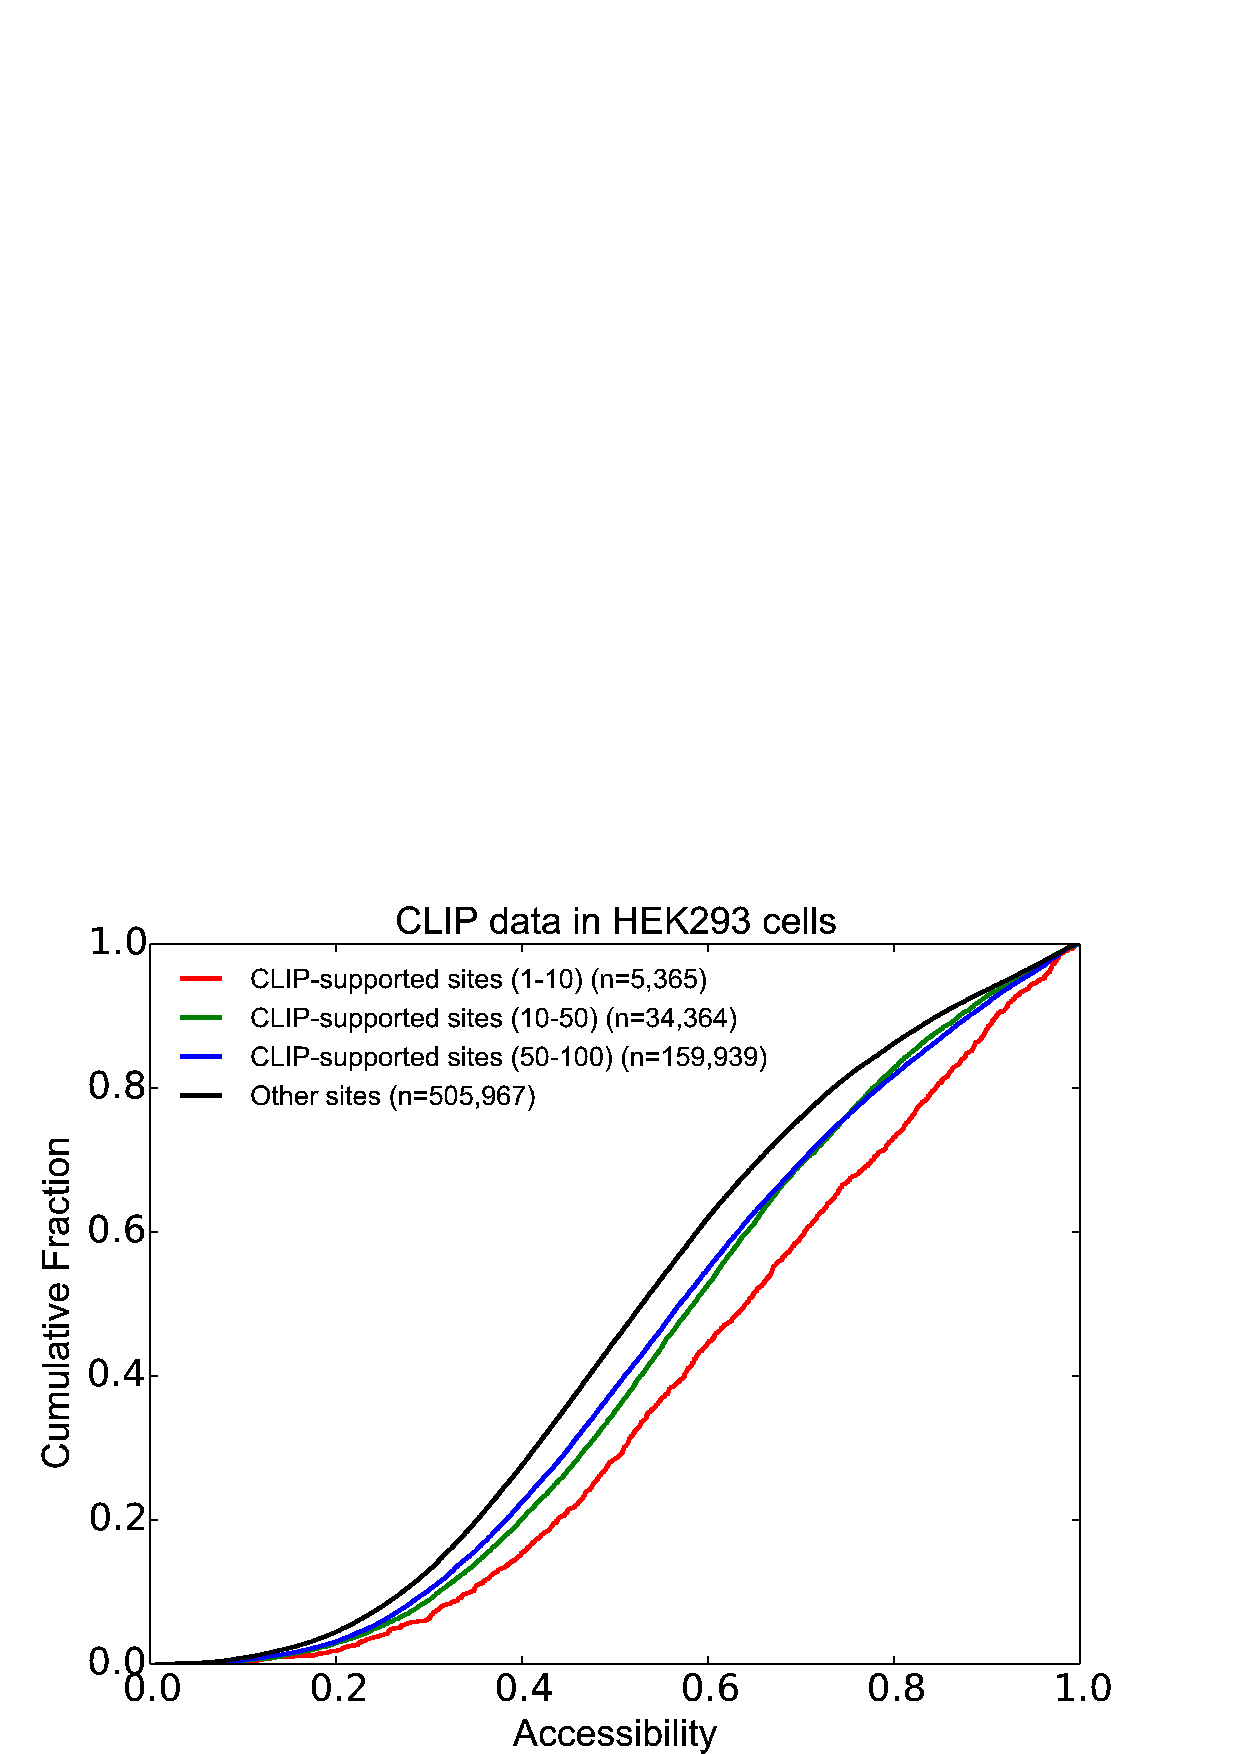
\includegraphics[width=0.55\textwidth,clip]{ch4_results_discussion/figures/Figure2a.pdf}
    \label{HuR_accessibility_HEK293}
}
\quad
	\subfloat[]{
	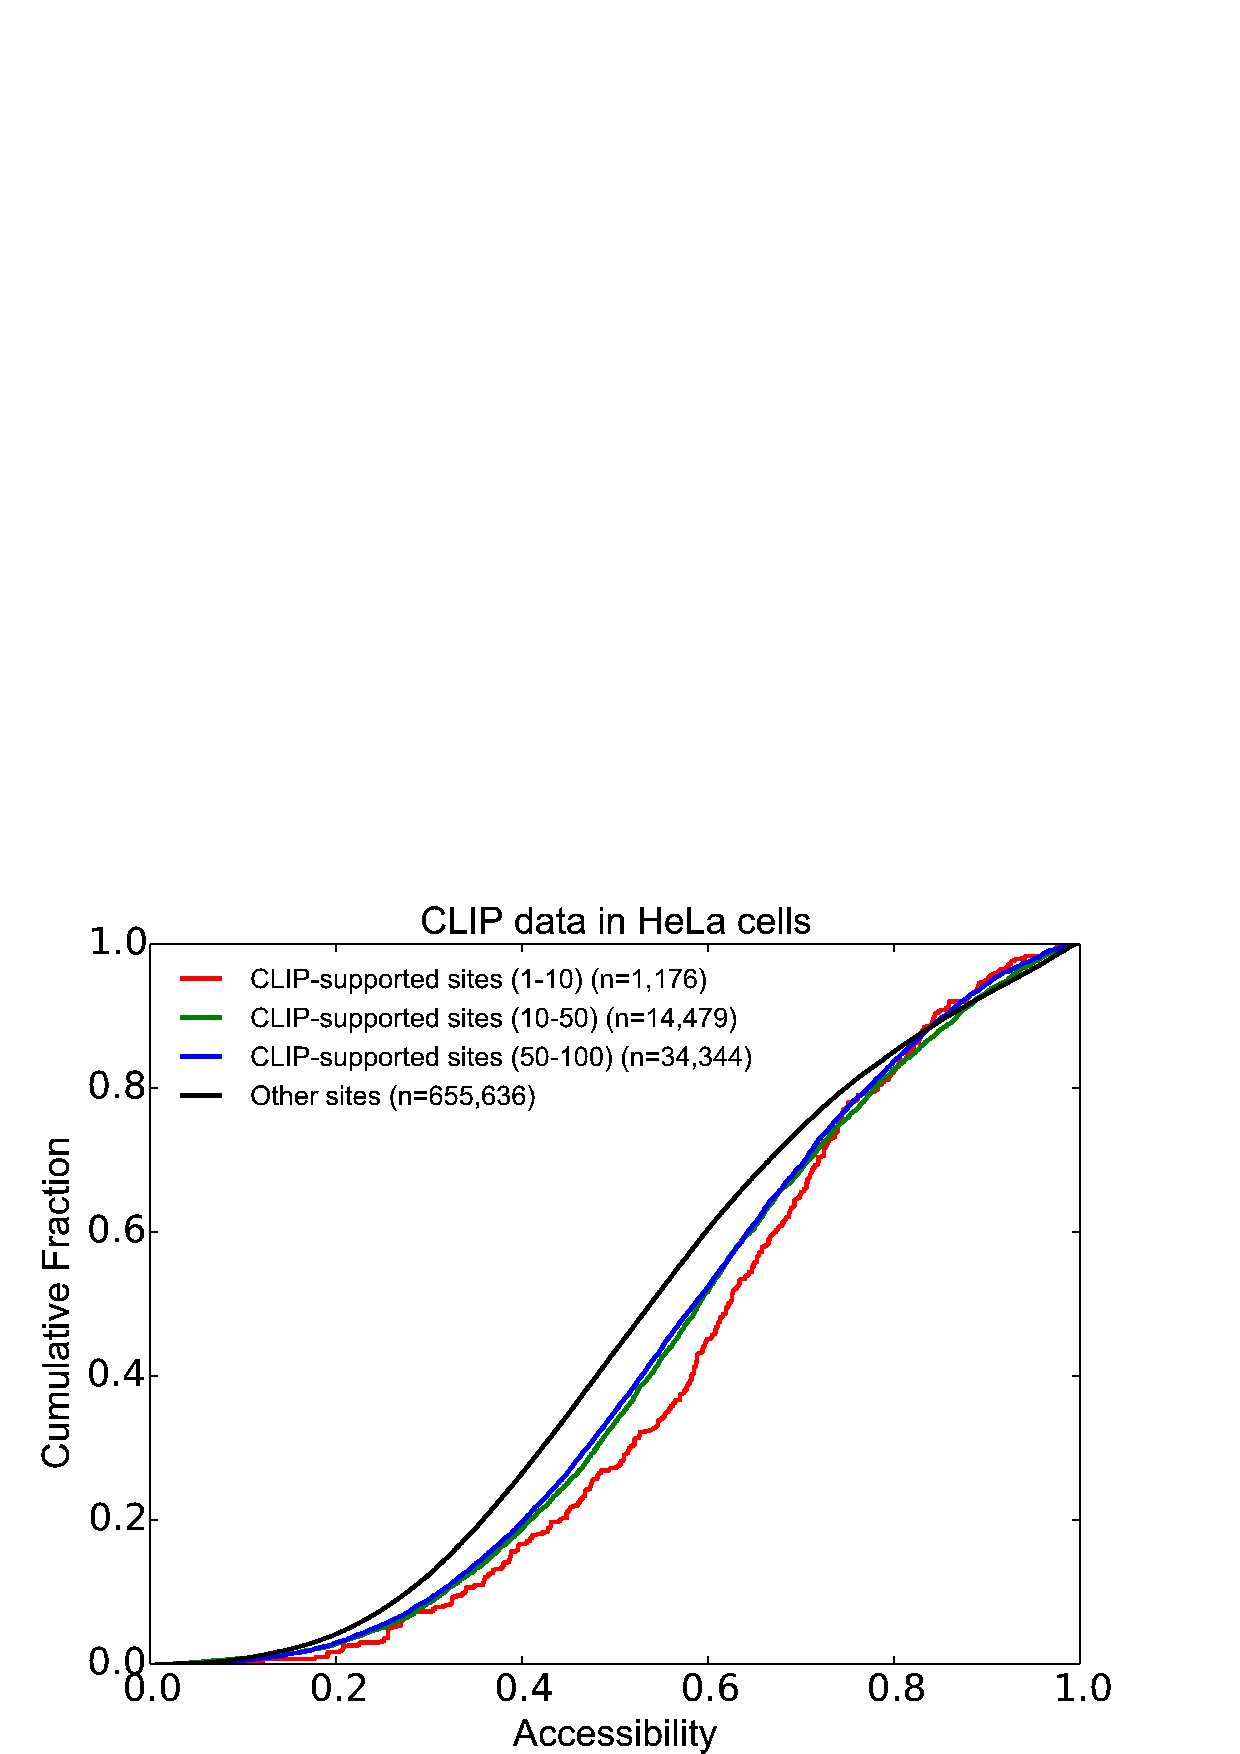
\includegraphics[width=0.55\textwidth,clip]{ch4_results_discussion/figures/Figure2b.pdf}
    \label{HuR_accessibility_HeLa}
}
\caption[Accessibility of HuR protein]{Comparison of CLIP-supported and not CLIP-supported sites (i.e., other sites) of HuR in terms of accessibility. For accessibility analysis, CLIP-supported sites are classified into different groups based on the scores of the peaks that they are located in. \subref{HuR_accessibility_HEK293} Cumulative density fraction of accessibility scores of CLIP-supported sites and other sites where CLIP experiment is performed in HEK293 cells. \subref{HuR_accessibility_HeLa} Cumulative density fraction of accessibility scores of CLIP-supported sites and other sites where CLIP experiment is performed in HeLa cells.}
\label{HuR_accessibility}
\end{figure}
%\shorthandon{=}

Either considering PARCLIP data from HEK293 cells \cite{hafner_10} or HeLa cells \cite{lebedeva_11}, we noticed that the CLIP-supported HuR sites are more accessible. This result is in accordance with previous studies \cite{hur_accessibility}. On the other hand, we grouped these CLIP-supported sites according to their peak score (i.e. percentiles downloaded from doRINA database) to see their effect in much detail and as expected, we noticed that the sites that reside in peaks with higher scores are more accessible compared to other CLIP-supported sites (MannWhitneyU two-tailed test P-value = $1.1E-203$ for HEK293 cells and P-value = $4.5E-35$ for HeLa cells)(See Figures \ref{HuR_accessibility_HEK293} and \ref{HuR_accessibility_HeLa}). Next, we repeated the same type of analysis to investigate the effect of PhastCons conservation scores on CLIP-supported sites. We observed that conservation scores significantly differ between CLIP-supported sites and other sites of HuR protein either considering HEK293 CLIP data (P-value = $6.1E-16$) or HeLa CLIP data (P-value $\approx 0$) (See Figures \ref{HuR_conservation_HEK293} and \ref{HuR_conservation_HeLa} respectively). The difference is much more significant in HeLa cells compared to HEK293 cells.

Figure \ref{PUM_accessibility} shows that PUM1(2) experimentally validated sites are less accessible compared to other sites (P-value = $1.74E-10$). PUM1 is known to bind single-stranded motifs \cite{wang_02} and to downregulate its target mRNAs. PUM2 is expected to have a similar binding preferences as PUM1. We considered PUM2 CLIP-supported sites for this analysis. However, as \ref{PUM_accessibility} shows, we observed the opposite where PUM2 CLIP-supported sites are less accessible compared to other sites. In order to investigate it in further detail, we distinguished CLIP-supported sites according to their peak scores. We observed that sites in the high scoring peaks (percentile 1-10) are less accessible compared to sites located in low scoring peaks (Percentile 50-100) with a P-value = $0.002$. Figure \ref{PUM_accessibility} shows the accessibility score distribution of sites in distinguished groups. In case of conservation, as shown in Figure ~\ref{PUM_conservation}, CLIP-supported sites are significantly more conserved than other sites (P-value $\approx 0$).

\clearpage
%\shorthandoff{=}
\begin{figure}[H]
	\centering
	\subfloat[]{
	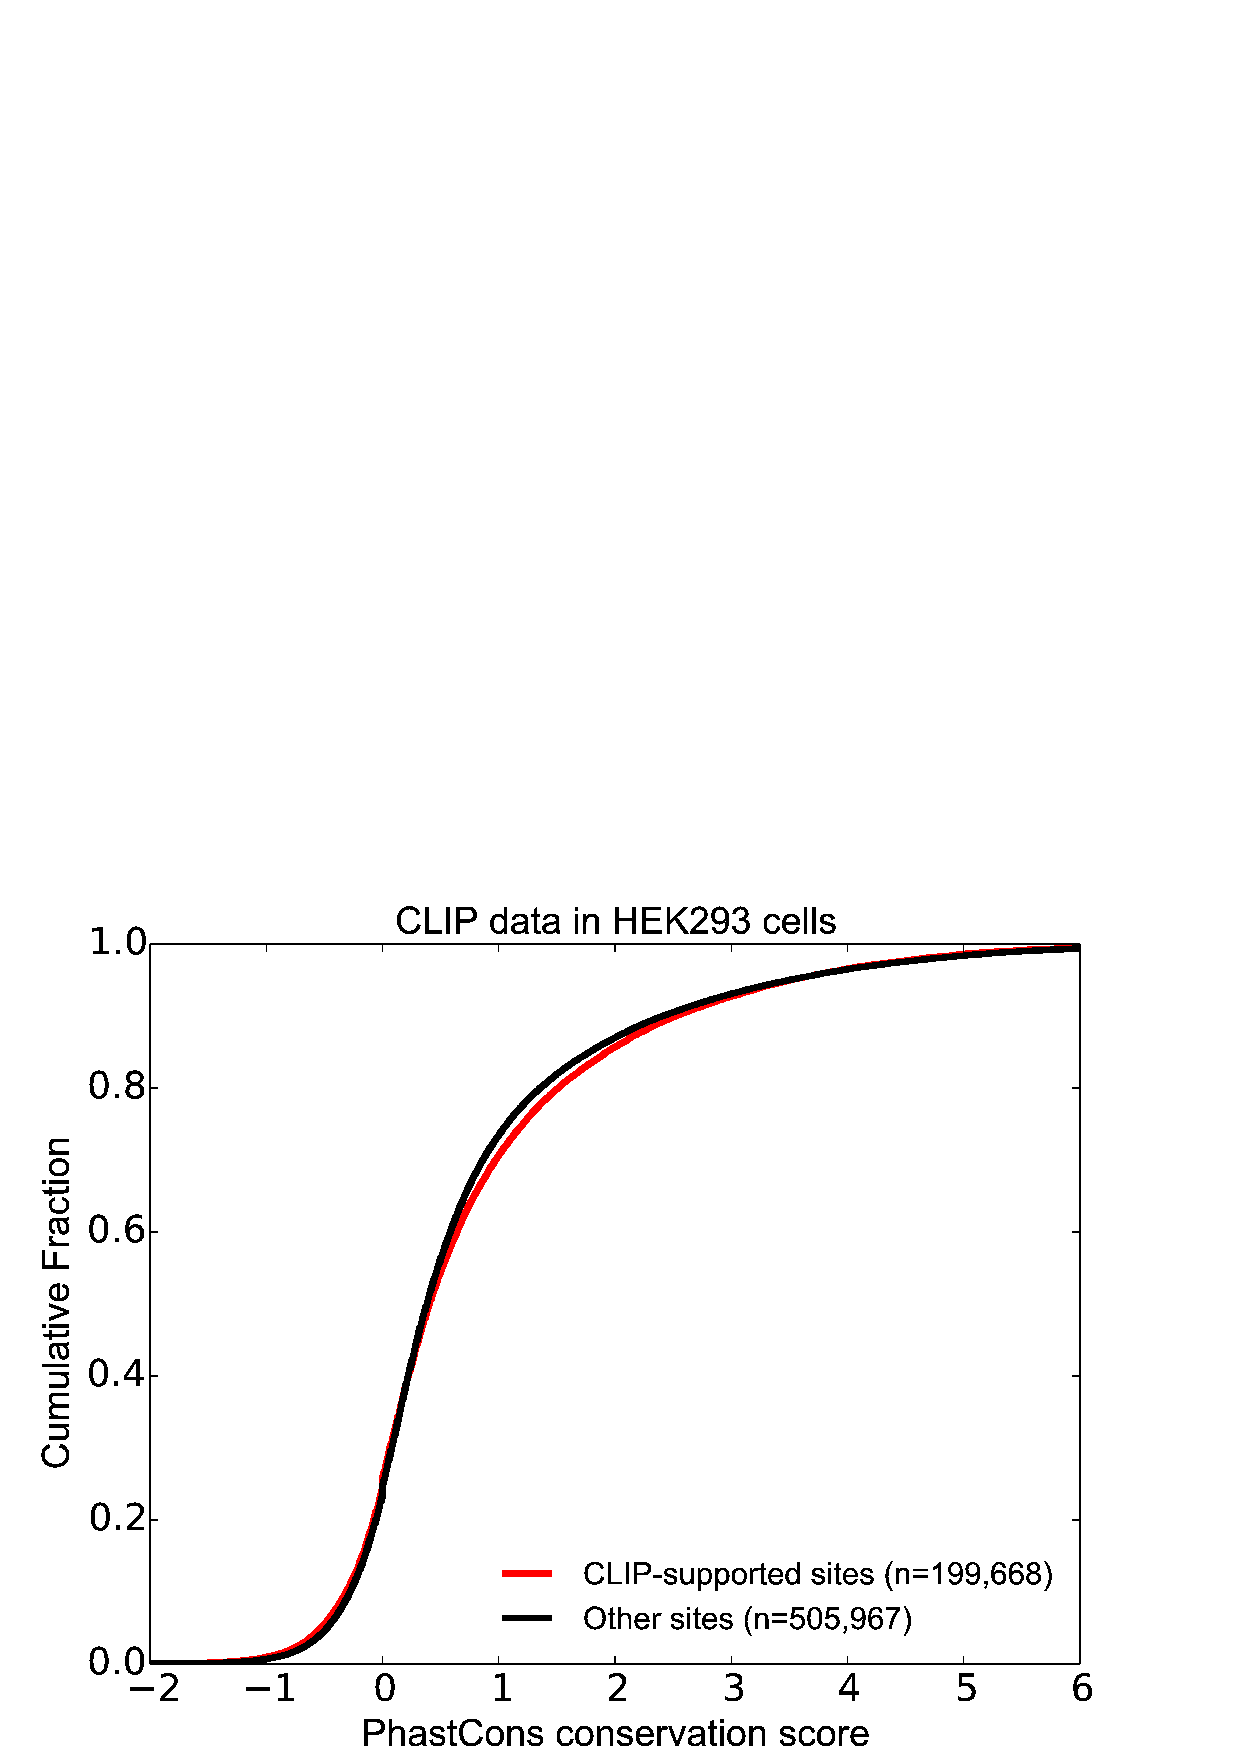
\includegraphics[width=0.7\textwidth,clip]{ch4_results_discussion/figures/Figure2c.pdf}
    \label{HuR_conservation_HEK293}
}
\quad
	\subfloat[]{
    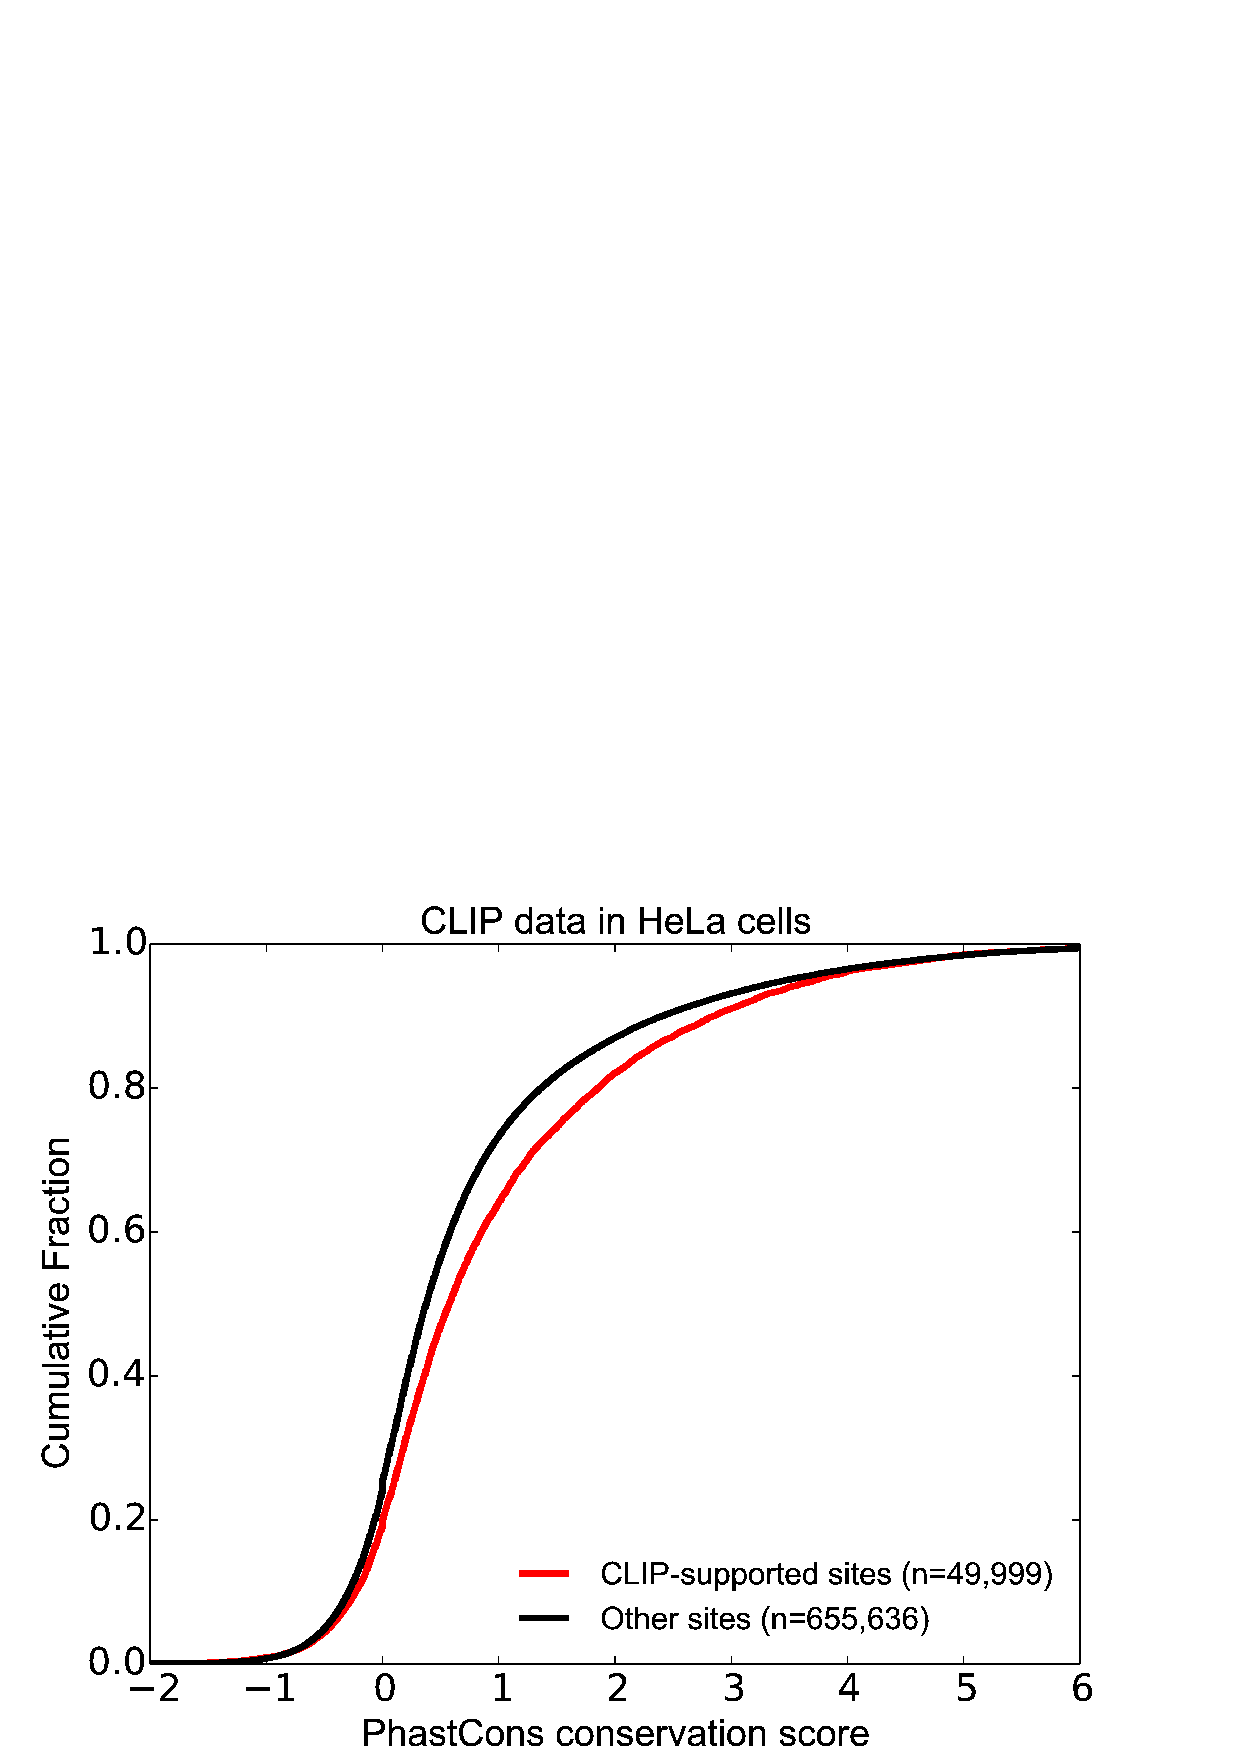
\includegraphics[width=0.7\textwidth,clip]{ch4_results_discussion/figures/Figure2d.pdf}
    \label{HuR_conservation_HeLa}
}
\caption[Conservation scores of HuR protein]{Comparison of CLIP-supported sites and not CLIP-supported sites (i.e., other sites) of HuR in terms of conservation scores. \subref{HuR_conservation_HEK293} Cumulative density fraction of conservation scores of CLIP-supported sites and other sites where CLIP experiment is performed in HEK293 cells. \subref{HuR_conservation_HeLa} Cumulative density fraction of conservation scores of CLIP-supported sites and other sites where CLIP experiment is performed in HeLa cells.}
\label{HuR_conservation}
\end{figure}
%\shorthandon{=}

\clearpage

%\shorthandoff{=}
\begin{figure}[H]
	\centering
	\subfloat[]{
    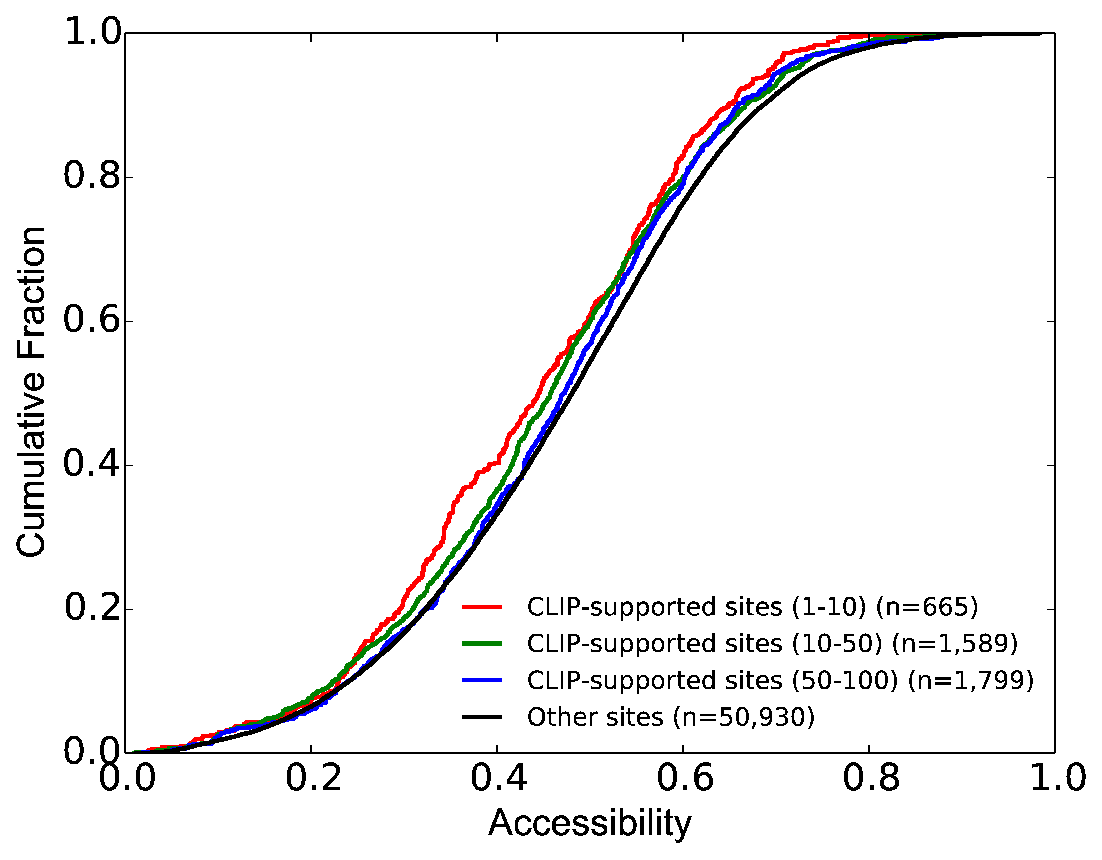
\includegraphics[width=0.7\textwidth,clip]{ch4_results_discussion/figures/Figure3a}
    \label{PUM_accessibility}
}
\quad
	\subfloat[]{
	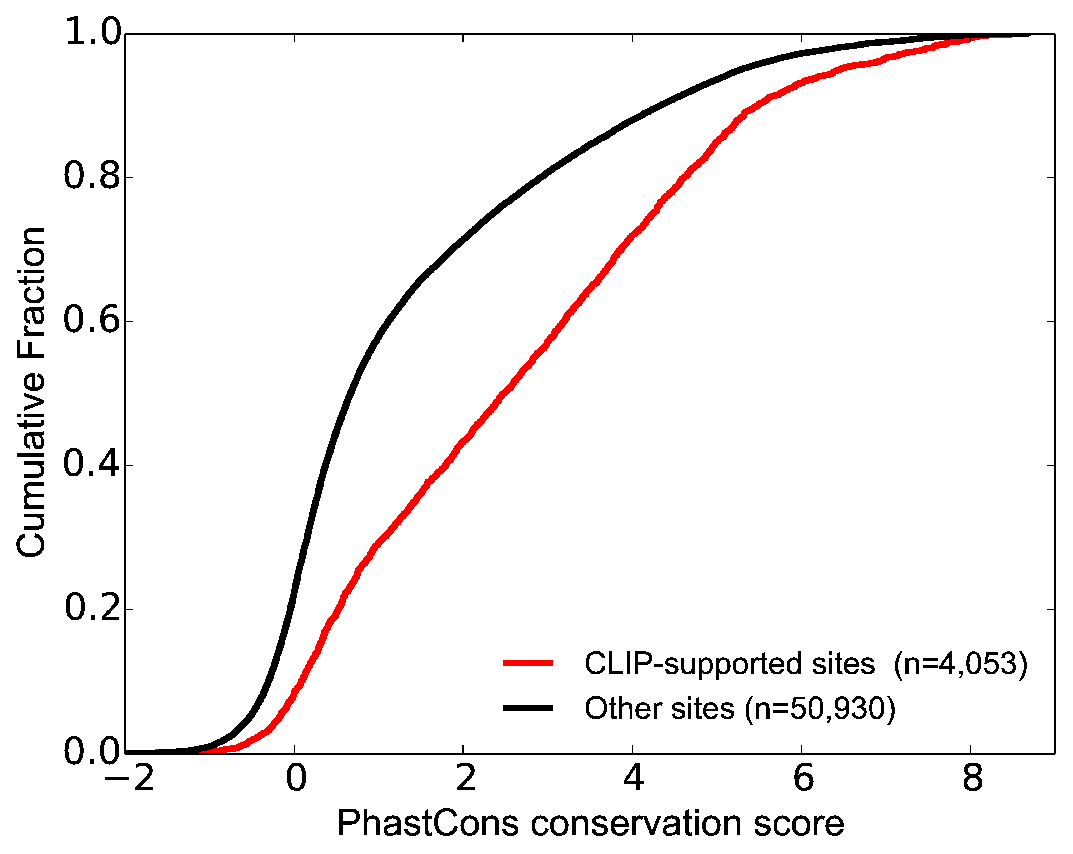
\includegraphics[width=0.7\textwidth,clip]{ch4_results_discussion/figures/Figure3b}
    \label{PUM_conservation}
}
\caption[Accessibility and conservation scores of PUM protein]{Comparison between CLIP-supported and other sites of PUM1(2) in terms of accessibility and conservation. \subref{PUM_accessibility} Cumulative density fraction of accessibility scores of CLIP-supported sites and other sites. \subref{PUM_conservation} Cumulative density fraction of conservation scores of CLIP-supported sites and other sites.}
\label{PUM_accessibility_and_conserv}
\end{figure}
%\shorthandon{=}

\clearpage
Furthermore, we repeated this analysis with QKI and IGF2BP1-3 RBPs. Figure \ref{IGF2BP_accessibility_and_conserv} shows that experimentally validated IGF2BP1-3 sites are more conserved compared to other sites (P-value = $4.4E-16$). On the other hand, in case of accessibility, we observed that CLIP-supported binding sites of IGF2BP1-3 are less accessible (P-value = $4.4E-16$). Figure \ref{QKI_accessibility_and_conserv} shows the comparison between CLIP-supported and other binding sites of QKI. We observed that CLIP-supported QKI binding sites are significantly more conserved compared to other QKI binding sites (P-value = $7.5E-09$). Besides, CLIP-supported QKI binding sites are more accessible (P-value = $2.7E-03$).

%\shorthandoff{=}
\begin{figure}[H]
	\centering
	\subfloat[]{
    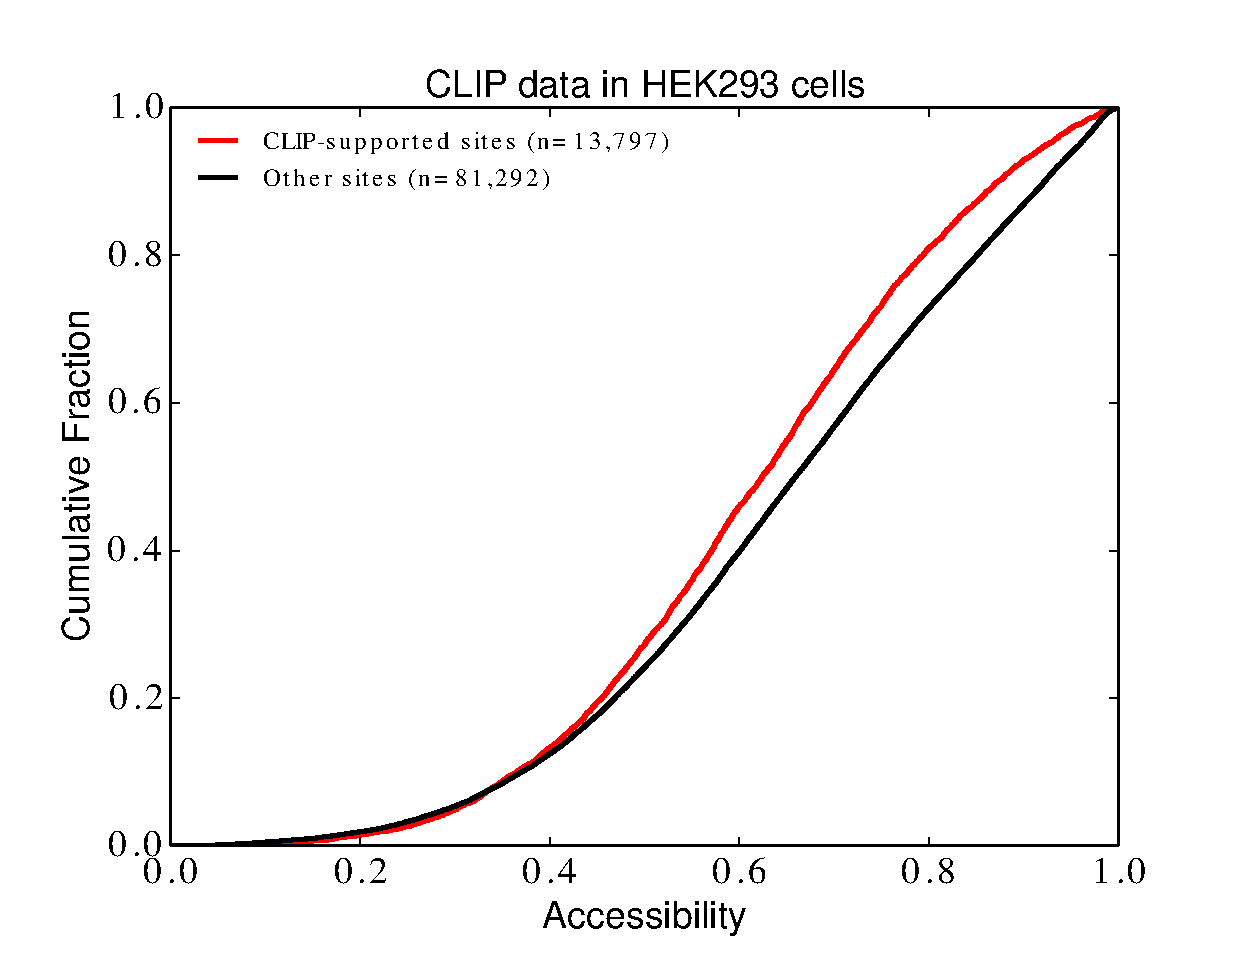
\includegraphics[width=0.65\textwidth,clip]{ch4_results_discussion/figures/IGF2BP_rnaplfold_accessibility_analysis_HEK293_2015_8_28.eps}
    \label{IGF2BP_accessibility}
}
\quad
	\subfloat[]{
	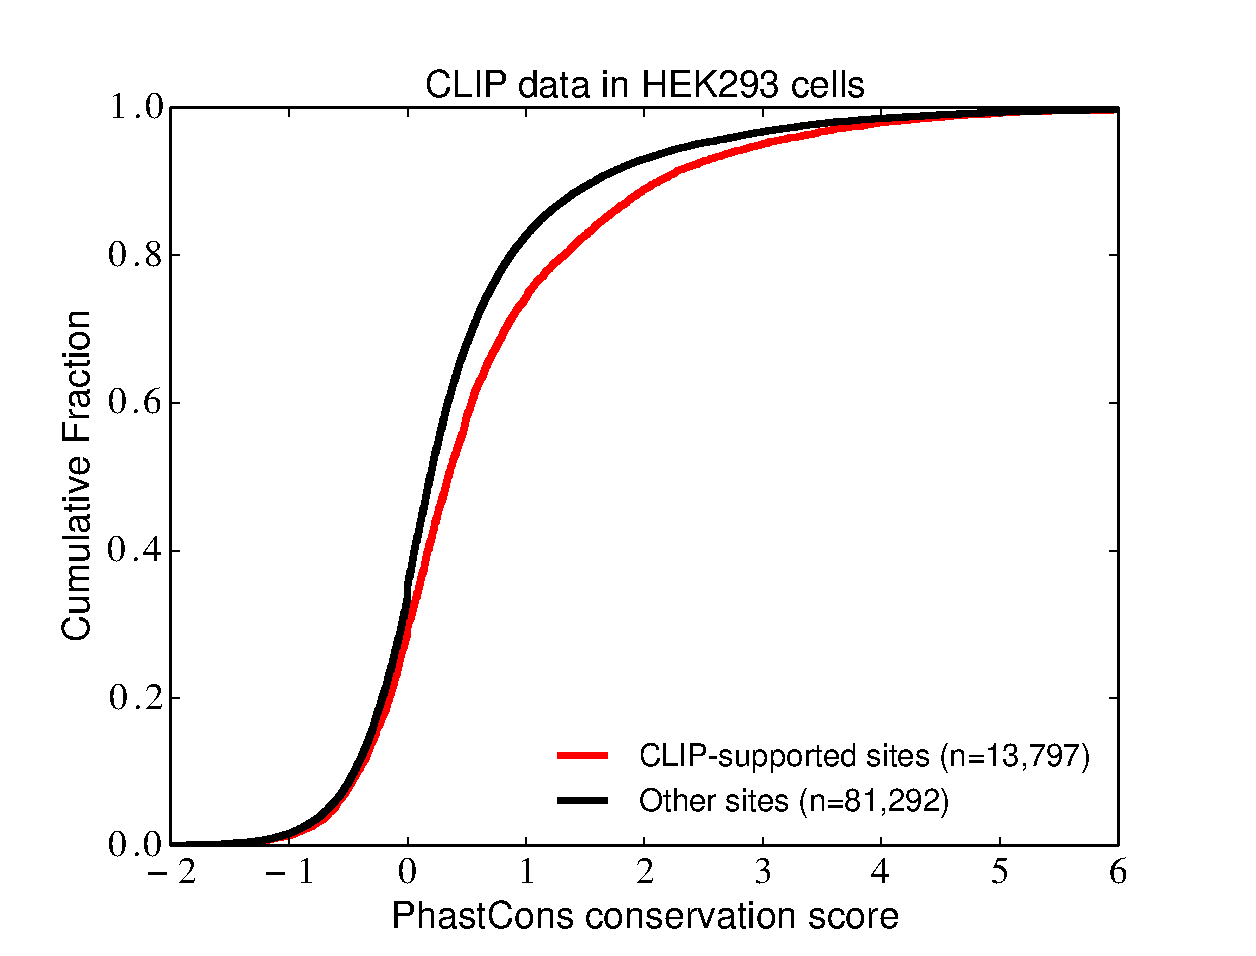
\includegraphics[width=0.65\textwidth,clip]{ch4_results_discussion/figures/IGF2BP_conservation_effect_HEK293_Aug27.eps}
    \label{IGF2BP_conservation}
}
\caption[Accessibility and conservation scores of IGF2BP1-3 protein]{Comparison between CLIP-supported and other sites of IGF2BP1-3 in terms of accessibility and conservation. \subref{IGF2BP_accessibility} Cumulative density fraction of accessibility scores of CLIP-supported sites and other sites. \subref{IGF2BP_conservation} Cumulative density fraction of conservation scores of CLIP-supported sites and other sites.}
\label{IGF2BP_accessibility_and_conserv}
\end{figure}
%\shorthandon{=}


%\shorthandoff{=}
\begin{figure}[H]
	\centering
	\subfloat[]{
    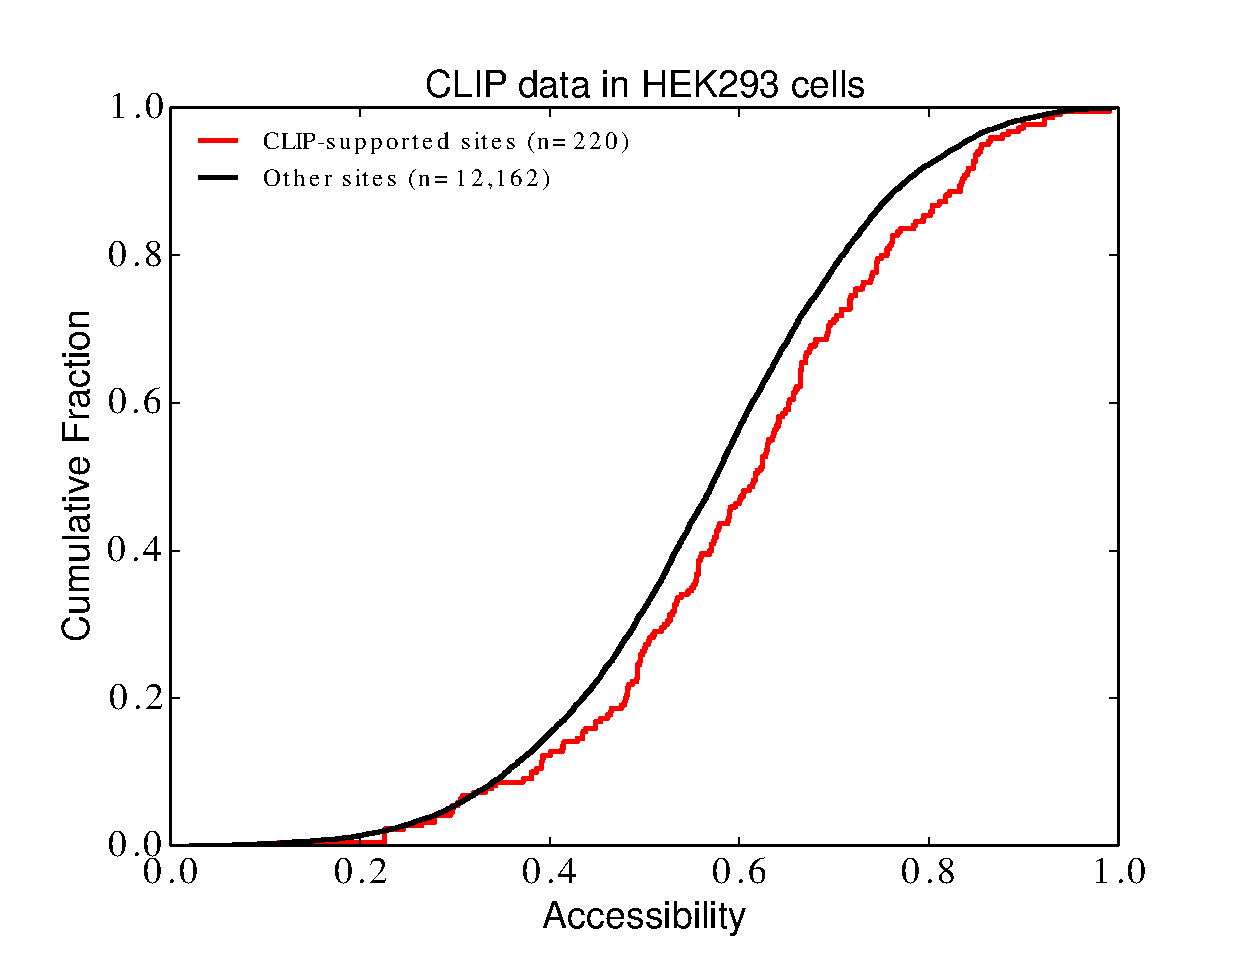
\includegraphics[width=0.65\textwidth,clip]{ch4_results_discussion/figures/QKI_rnaplfold_accessibility_analysis_HEK293_2015_8_28.eps}
    \label{QKI_accessibility}
}
\quad
	\subfloat[]{
	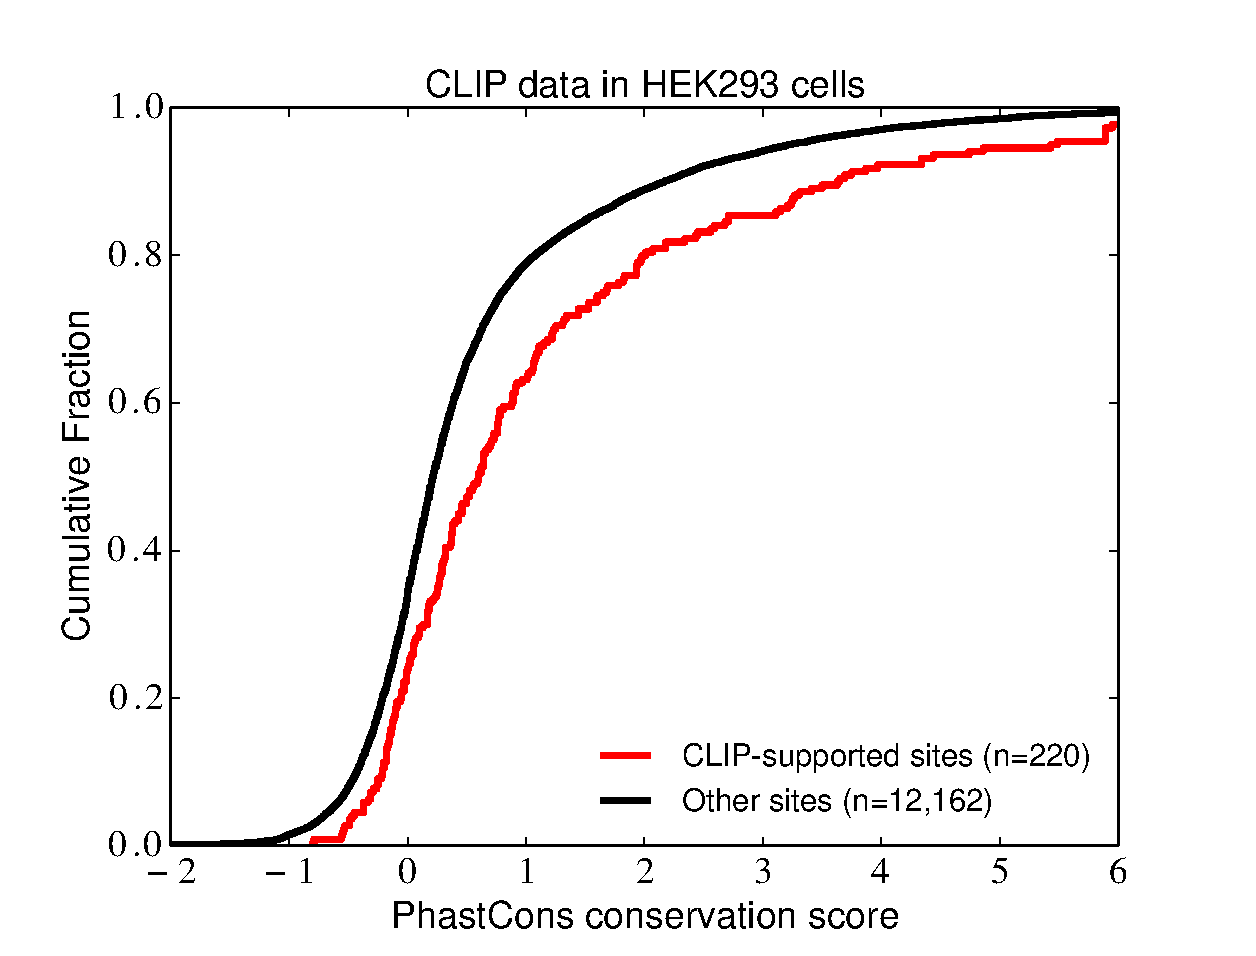
\includegraphics[width=0.65\textwidth,clip]{ch4_results_discussion/figures/QKI_conservation_effect_HEK293_Aug27.eps}
    \label{QKI_conservation}
}
\caption[Accessibility and conservation scores of QKI protein]{Comparison between CLIP-supported and other sites of QKI in terms of accessibility and conservation. \subref{QKI_accessibility} Cumulative density fraction of accessibility scores of CLIP-supported sites and other sites. \subref{QKI_conservation} Cumulative density fraction of conservation scores of CLIP-supported sites and other sites.}
\label{QKI_accessibility_and_conserv}
\end{figure}
%\shorthandon{=}

As discussed before, we distinguished CLIP-supported sites of PUM2 and HuR according to their CLIP score in accessibility analysis. However, in case of QKI and IGF2BP1-3 binding sites, we considered all CLIP-supported binding sites in one single group. That is because there are little amount of CLIP-supported binding sites and distinguishing them into several groups makes it harder to investigate the effect of CLIP-supported sites in case of accessibility and conservation.

Generally, we investigated the effect of CLIP-supported sites of RBPs in case of accessibility and conservation. In the following section, we utilize knockdown datasets to further investigate effect of CLIP-supported sites on expression of mRNAs.

%change the title
\section{Analysis of knockdown datasets}

In this series of analyses we aim to assess the effect of CLIP-supported sites and consequences of competition between particular RBPs and other factors on the expression of mRNAs. We repeated this analysis for HuR, QKI, and IGF2BP1-3 proteins for which knockdown datasets are available. We used log fold expression changes of transcripts upon HuR depletion in HEK293 and HeLa cells from \cite{mukharjee_11} and \cite{lebedeva_11} respectively. As for QKI and IGF2BP1-3, we used knockdown datasets from Hafner et al. in HEK293 cells \cite{hafner_10}.

Mukharjee et al. \cite{mukharjee_11} has shown that even transcripts with only intronic HuR sites still show reduced expression upon HuR knockdown in HEK293 cells. Our aim is to understand the function of HuR sites in 3'UTs. Therefore, we decided to filter out those transcripts that contain intronic HuR sites in order to avoid their concealed effects throughout the following analyses related to HuR.

\subsection{Effect of CLIP-supported sites on transcripts expression}
 
In this analysis our aim was to investigate the effect of experimentally validated RBP sites on expression of transcripts compared to the effect of other sites of that RBP which are not CLIP-supported. Expression log fold changes upon knockdown of a single factor provides valuable information about that factor's behavior. HuR increases the stability of its target mRNAs. Therefore, we expected to see higher destabilization in transcripts containing experimentally validated HuR sites compared to other sites in which HuR was knocked down.

In order to illustrate our expectations, we classified transcripts into three groups: (i) those that have at least one CLIP-supported HuR site; (ii) those that have one or more predicted HuR sites but none of them are CLIP-supported; and (iii) those that have no HuR sites at all. Figure ~\ref{HuR_CLIPsupport} shows the cumulative distribution of LFC of the transcripts belonging to these groups. Considering the distribution of LFC of the transcripts having no HuR sites at all as our baseline, we observed that transcripts in the first group are more destabilized upon HuR Knockdown compared to those transcripts in the second group. (Figure \ref{HuR_CLIPsupport_HEK293}, P-value = $1.8E-81$) and  (Figure \ref{HuR_CLIPsupport_HeLa}, P-value = $5.2E-05$)

\clearpage
%\shorthandoff{=}
\begin{figure}[H]
	\centering
	\subfloat[]{
	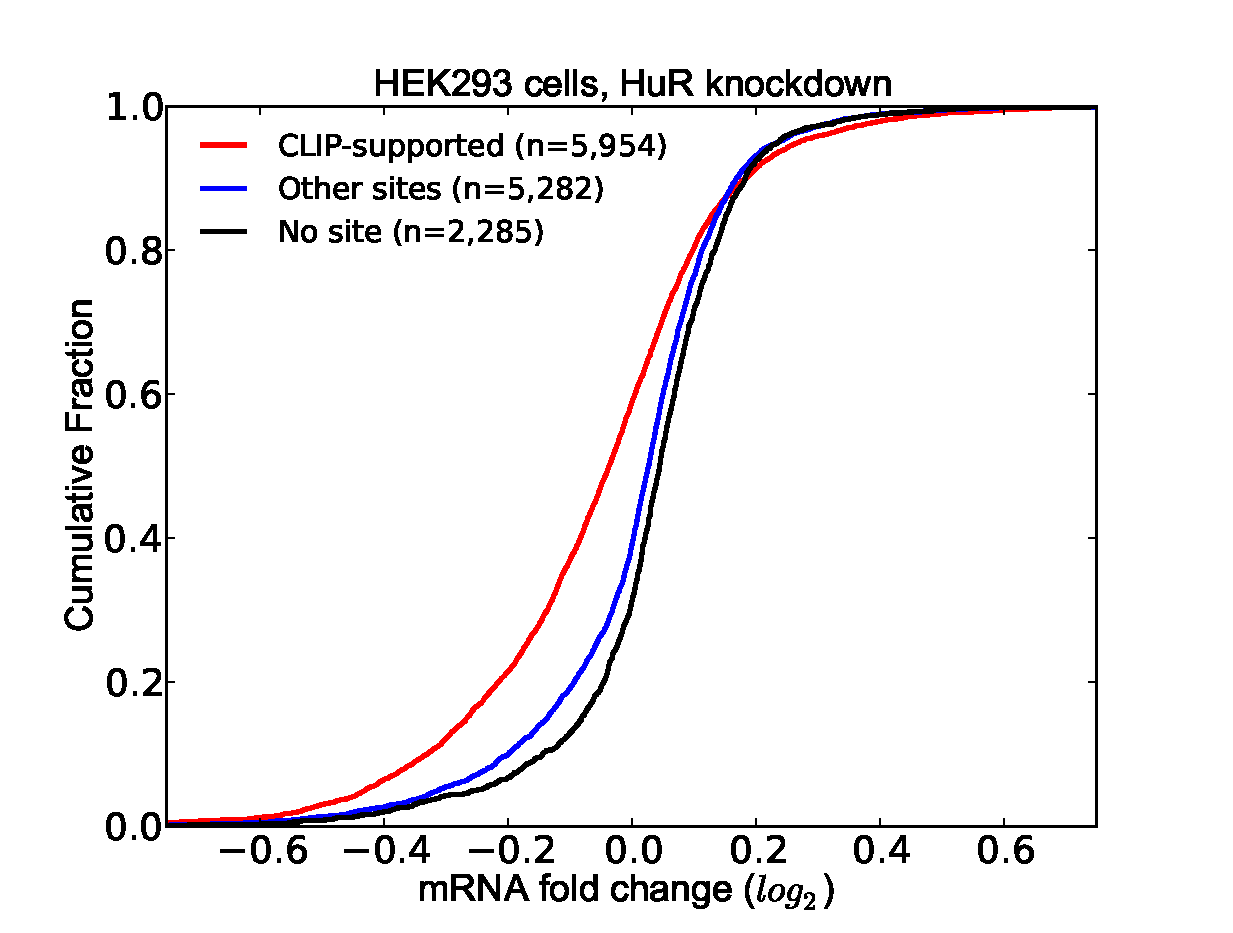
\includegraphics[width=0.65\textwidth,clip]{ch4_results_discussion/figures/Mukharjee_HEK293_CLIP_supported_notsupported_HuRAll_ConsTHNone_Excluded_allgroups_2015_8_20.eps}
    \label{HuR_CLIPsupport_HEK293}
}
\quad
	\subfloat[]{
    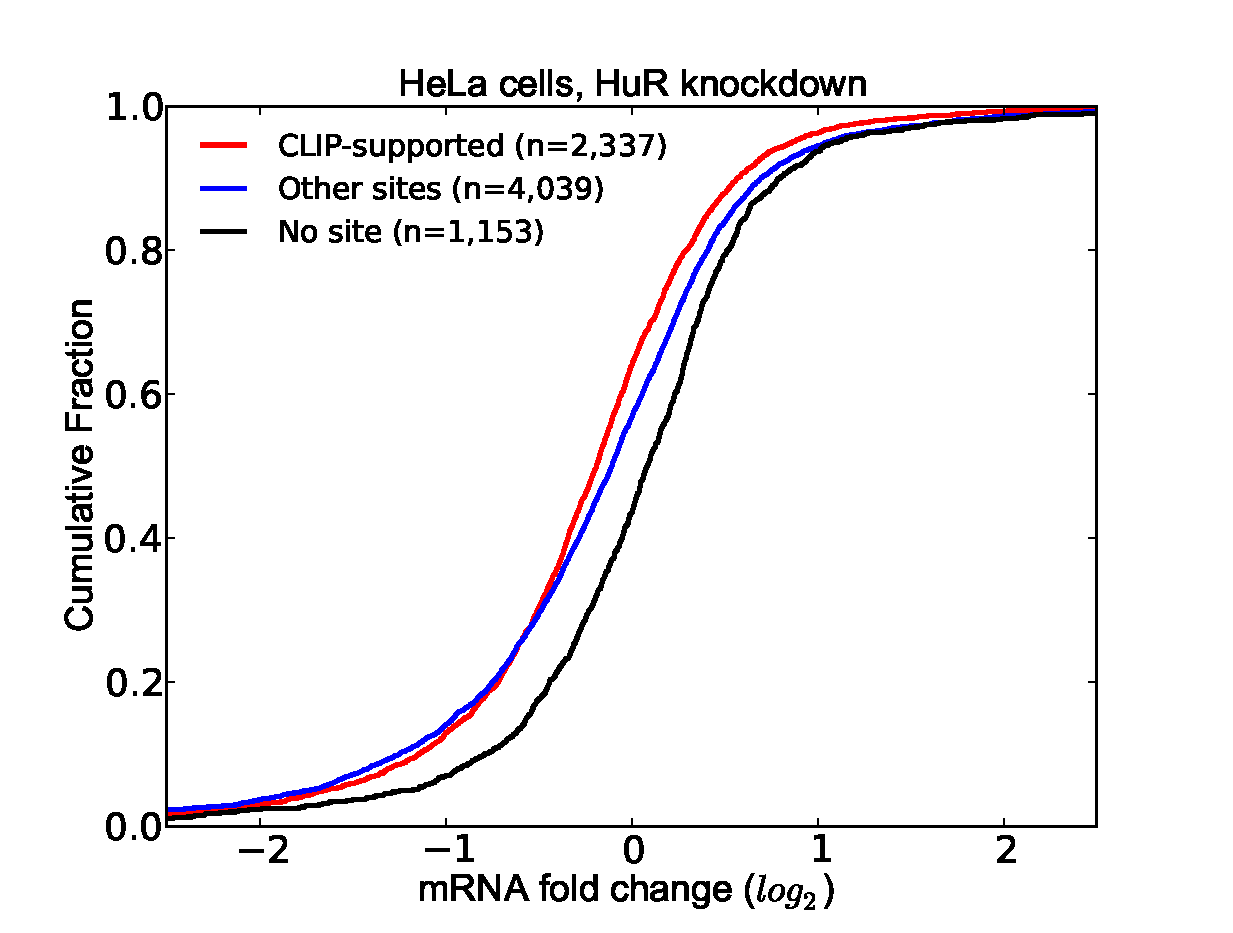
\includegraphics[width=0.65\textwidth,clip]{ch4_results_discussion/figures/Lebedeva_HeLa_CLIP_supported_notsupported_HuRAll_ConsTHNone_Excluded_allgroups_2015_8_20.eps}
    \label{HuR_CLIPsupport_HeLa}
}
\caption[Comparison between CLIP-supported HuR sites and Other sites]{Comparison of the effect of HuR depletion on transcripts that contain CLIP-supported HuR sites against those that do not contain CLIP-supported HuR sites. X axis shows the log fold change of transcripts upon HuR depletion. \subref{HuR_CLIPsupport_HEK293} Response of mRNAs to the loss of HuR in HEK293 cells. \subref{HuR_CLIPsupport_HeLa} Response of mRNAs to the loss of HuR in HeLa cells. }
\label{HuR_CLIPsupport}
\end{figure}
%\shorthandon{=}

We also repeated this analysis with QKI and IGF2BP1-3 RBPs in order to further approve our findings with HuR. Figure \ref{QKI_CLIP-supported} shows the comparison between expression of transcripts that contain CLIP-supported QKI binding sites and those that do not contain CLIP-supported QKI binding sites in case of QKI knockdown. Hafner et al. \cite{hafner_10} provides two siRNA dataset for QKI knockdown and here we calculated the average values from these two siRNA knockdown datasets and used it to investigate the effect of CLIP-supported QKI binding sites on expression of their target mRNAs. 

%\shorthandoff{=}
\begin{figure}[H]
	\centering
	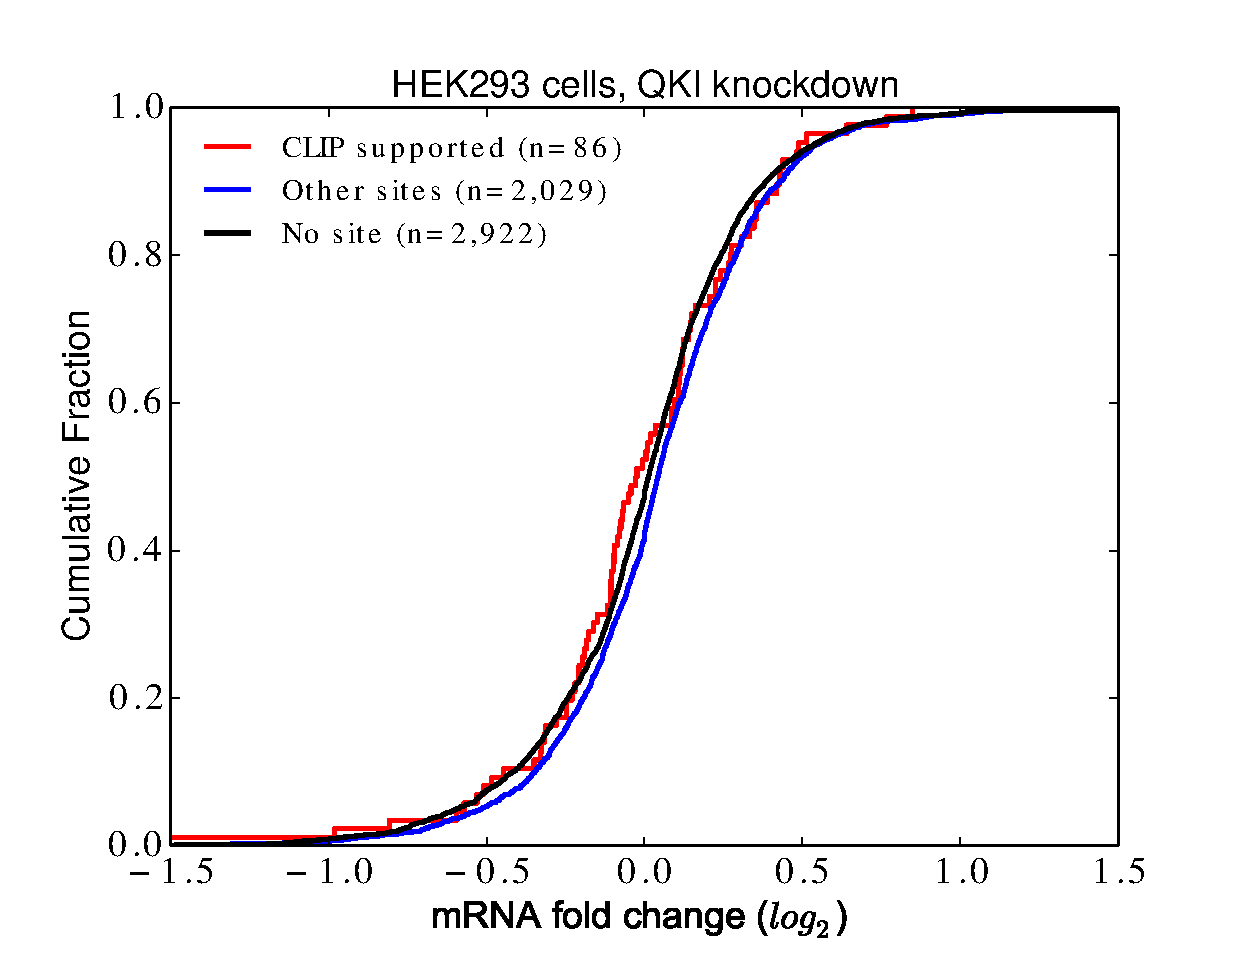
\includegraphics[width=0.8\textwidth,clip]{ch4_results_discussion/figures/Hafner_HEK293_QKI_SetAB_avg_CLIP_supported_notsupported_THNone_corrected_2015_8_28.eps}
\caption[Comparison between CLIP-supported QKI sites and other sites]{Comparison of the effect of QKI depletion on transcripts that contain CLIP-supported QKI sites against those that do not contain CLIP-supported QKI sites. X axis shows the log fold change of transcripts upon QKI depletion. It shows the response of mRNAs to the loss of QKI in HEK293 cells}
\label{QKI_CLIP-supported}
\end{figure}
%\shorthandon{=}

%\shorthandoff{=}
\begin{figure}[H]
	\centering
	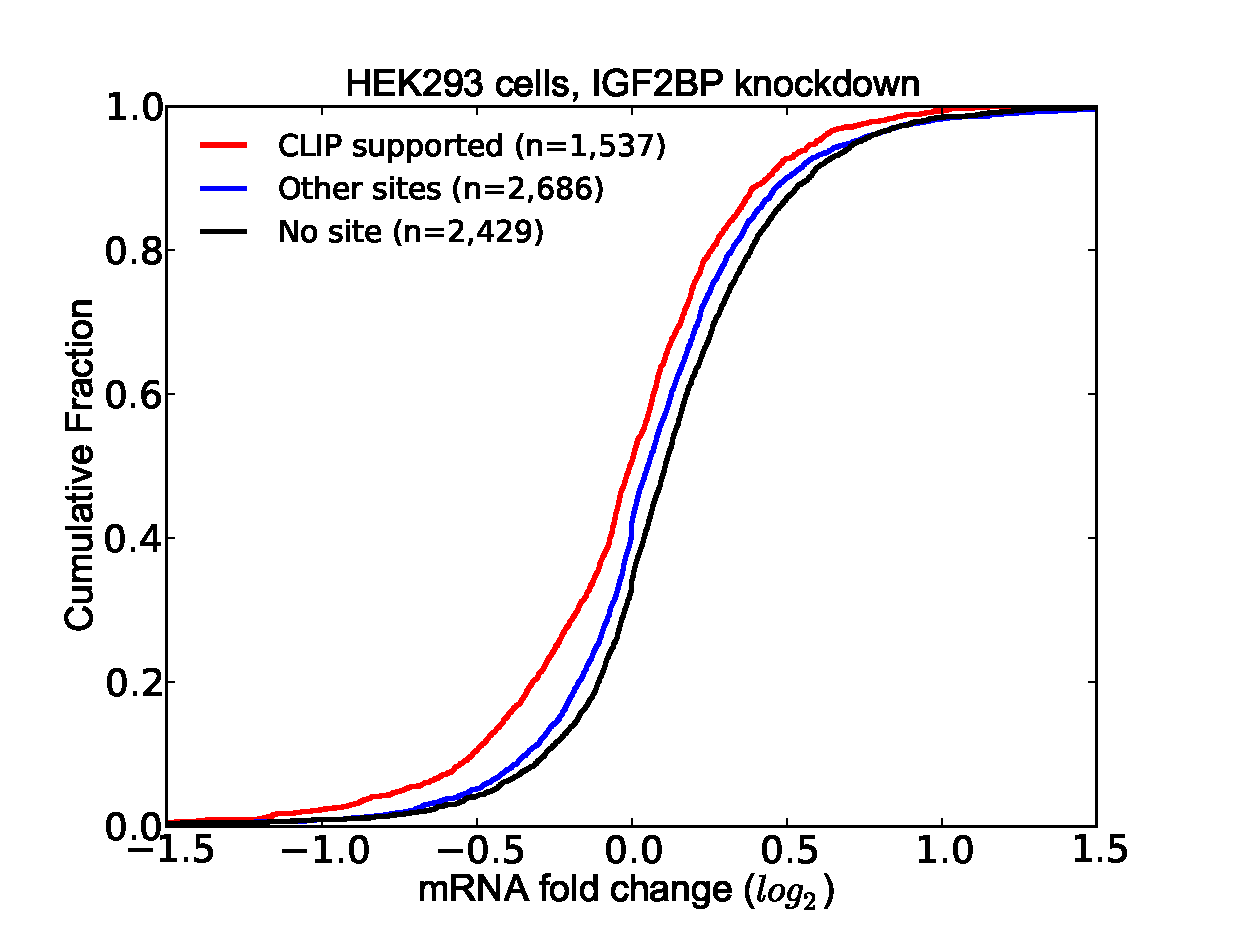
\includegraphics[width=0.8\textwidth,clip]{ch4_results_discussion/figures/Hafner_HEK293_IGF2BP1-2_CLIP_supported_notsupported_THNone_2015_8_28_corrected.eps}
\caption[Comparison between CLIP-supported IGF2BP1-3 sites and other sites]{Comparison of the effect of IGF2BP1-3 depletion on transcripts that contain CLIP-supported IGF2BP1-3 sites against those that do not contain CLIP-supported IGF2BP1-3 sites. X axis shows the log fold change of transcripts upon IGF2BP1-3 depletion. It shows the response of mRNAs to the loss of IGF2BP1-3 in HEK293 cells}
\label{IGF_CLIP-supported}
\end{figure}
%\shorthandon{=}

As figure \ref{QKI_CLIP-supported} shows, we couldn't observe a net effect on the expression of QKI target mRNAs. There is no significant difference between log fold change of transcripts in groups 1 and 2 (P-value = $0.17$). Indeed, the roles of QKI on splicing is well established; however, its effect to stability is not well determined. Hafner et al. \cite{hafner_10} has found that QKI decreases stability. On the other hand, another study by Teplova et al. \cite{teplova_2013} have analyzed the same datasets and showed that QKI increases stability. Therefore, we decided to exclude this RBP from our analyses.

Figure \ref{IGF_CLIP-supported} shows the effect of CLIP-supported IGF2BP1-3 sites on abundance of its target mRNAs. IGF2BP1-3 is known to increase the stability of its target mRNAs. Indeed, we observed that the transcripts which contain CLIP-supported IGF2BP1-3 binding sites are more destabilized upon IGF2BP1-3 knockdown compared to transcripts in second group (P-value = $6.84E-14$).

\subsection{The effect of competition to HuR function}

Transcripts are known to be occupied by several RBPs and miRNAs concurrently. In this analysis, we aim to determine the outcome of HuR competition with other factors. We suppose that two factors may involve in a competitive situation when they both target the same region. If the binding sites of these factors overlap with each other, we consider them as putative competitors. As such, In the initial step, we defined a HuR site to be overlapping if there was another factor (RBP or miRNA) which targets the same region. Next, we classified the transcripts into three groups: (i) transcripts that have at least one CLIP-supported HuR site that is not overlapping with any other site (no competition); (ii) transcripts that have at least one CLIP-supported HuR site but all HuR sites including the CLIP-supported ones are overlapping with sites of other factors (competition); and (iii) transcripts that have no HuR site at all. In order to filter out the effect of transcripts that contain intronic HuR sites, we excluded them in the initial step. Figure \ref{HuR_competition} illustrates that transcripts in \textit{no competition} group are destabilized more after HuR knockdown compared to the transcripts in \textit{competition} group. This observation holds true for HuR knockdown dataset both from HEK293 and HeLa cell lines. (P-value = $1.4E-05$ and $7.5E-05$ respectively)

\clearpage
%\shorthandoff{=}
\begin{figure}[H]
	\centering
	\subfloat[]{
	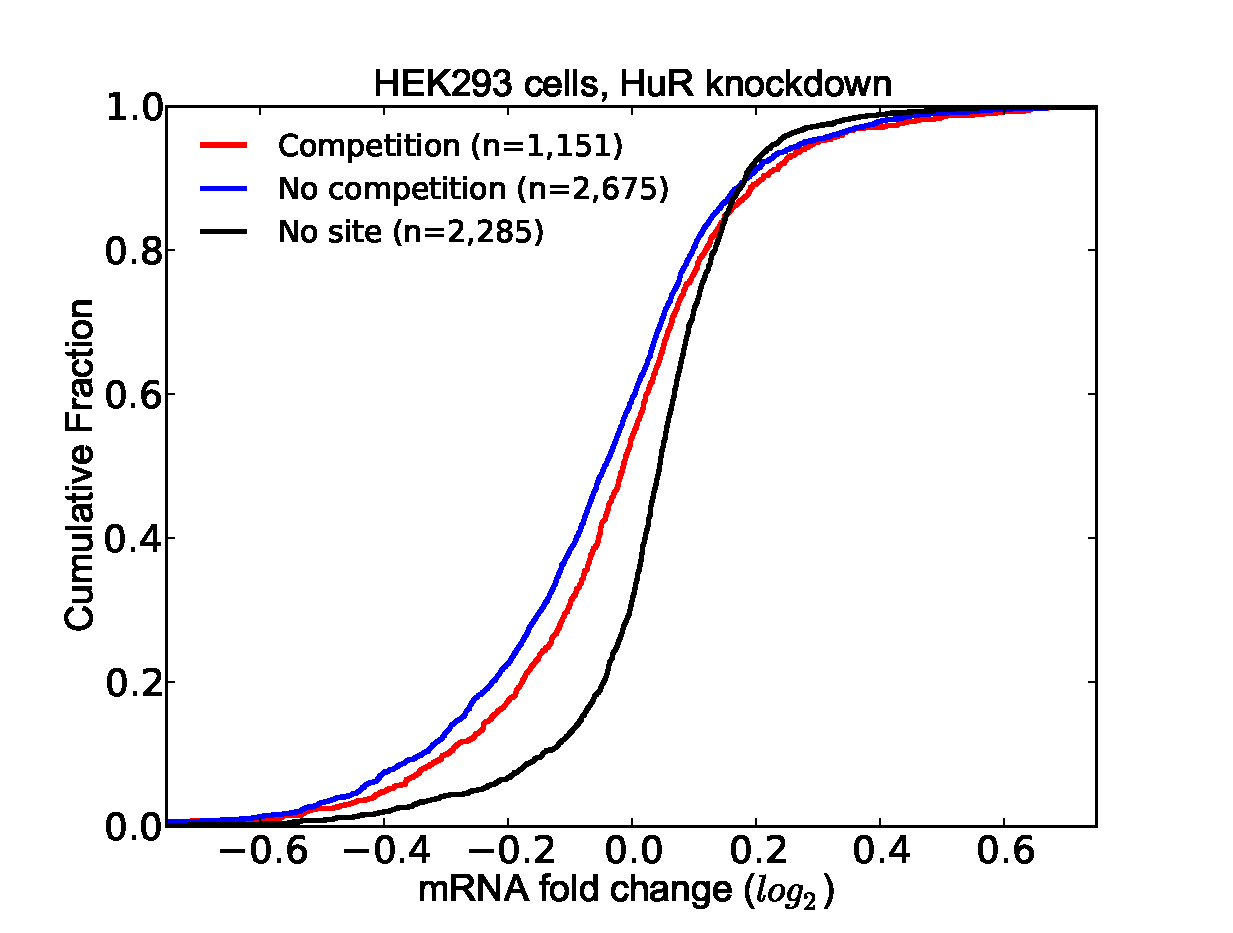
\includegraphics[width=0.75\textwidth,clip]{ch4_results_discussion/figures/HuR_Mukharjee_HEK293_competition_allsites_ConsTHNone_overlap_ExcludedAll_Expressedtop1002015_8_20.eps}
    \label{HuR_competition_HEK293}
}
\quad
	\subfloat[]{
    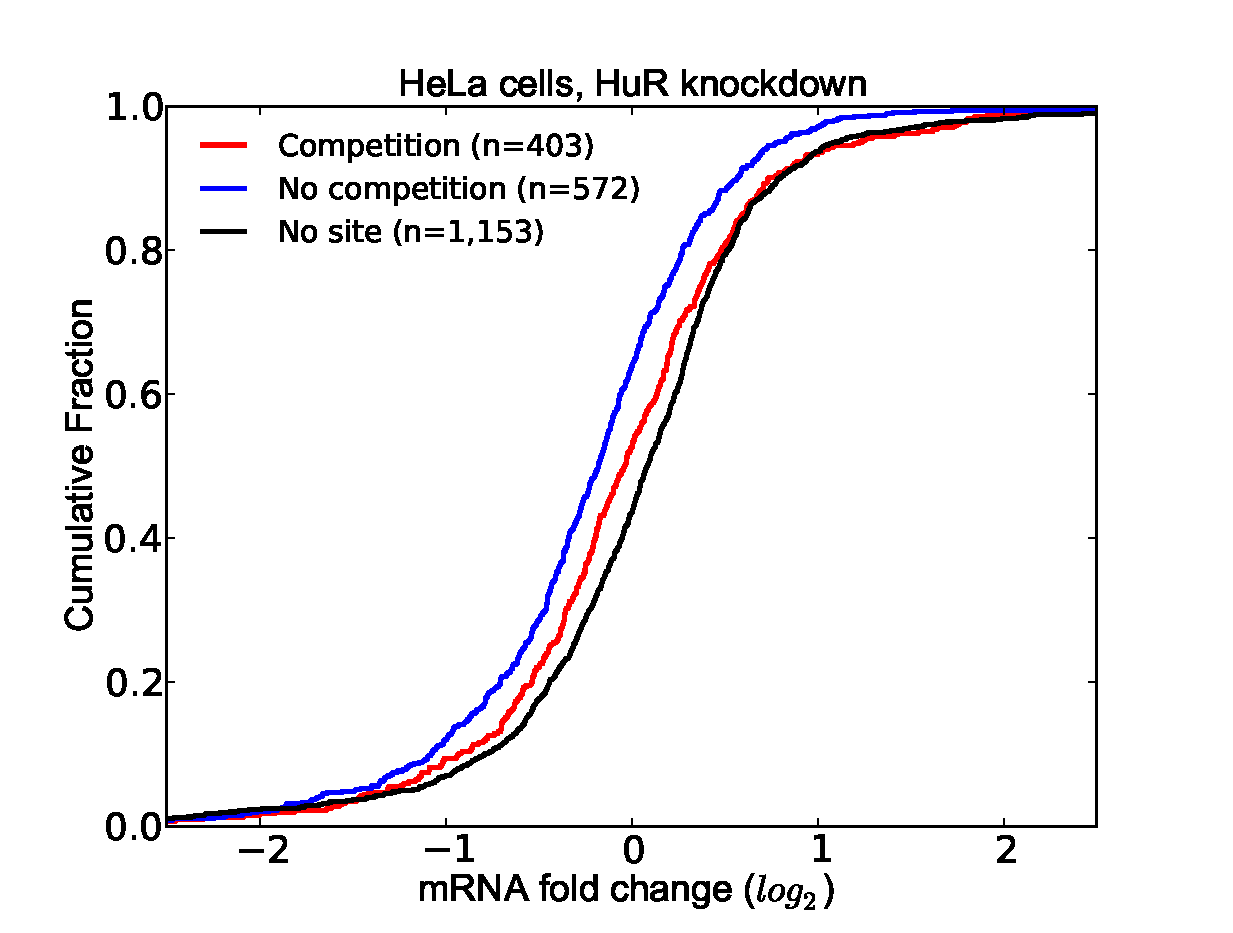
\includegraphics[width=0.75\textwidth,clip]{ch4_results_discussion/figures/HuR_Lebedeva_HeLa_competition_allsites_ConsTHNone_overlap_ExcludedAll_Expressedtop1002015_8_20.eps}
    \label{HuR_competition_HeLa}
}
\caption[Competition effect on HuR sites]{The effect of competition between HuR binding sites and other factors binding sites on expression of mRNAs. \subref{HuR_competition_HEK293} Response of mRNAs to the loss of HuR in HEK293 cells. \subref{HuR_competition_HeLa} Response of mRNAs to the loss of HuR in HeLa cells.}
\label{HuR_competition}
\end{figure}
%\shorthandon{=}

Here, we assess the effect of competition of HuR binding sites with other factors. We demonstrated that transcripts where all HuR binding sites are in competition with other factors, show less change in case of expression upon HuR knockdown.

\section{Analysis of co-occurrence of motifs}

%In this set of analysis we aim to determine whether sites of a pair of factors (RBP and miRNA) co-occur within a certain distance more often than expected by chance. We followed a similar method discussed in Jiang et al. \cite{jiang_13} At first step, for each site of a factor, we calculated the number of neighboring sites of other factors in each 50-nt-window 500-nt on either side of the site. Next, we calculated the impractical P-value by comparing this count to the distribution of counts obtained when factor identities are shuffled 10000 times (keeping the site positions fixed). We repeated this permutation test three times, using different shuffling types: (i) shuffling the factor identities of sites that are located on the same chromosome; (ii) classifying the sites into three groups based on AU-content (i.e., $<3$,  $\geq 3$ and $< 6$, $\geq 6$ ) and shuffling the factor identities of the sites in the same group; (iii) classifying the sites into 10 groups according to their relative position within the 3'UTRs and shuffling the factor identities of the sites in the same group (see \cite{jiang_13} for more details). In order to correct the P-values for multiple testing, we converted them into q-values which are a measure of significance in terms of false discovery rate rather than the false positive rate \cite{qvalue}. After calculating the q-values, for each interested factor, we defined its interacting factors. we considered a factor as an interacting one when it has at least one window with q-value less than 0.05 in each permutation test.
In this set of analysis we aim to determine whether sites of a pair of factors (RBP and miRNA) co-occur within a certain distance more often than expected by chance. As discussed in the methods chapter, we calculated the impractical P-value for each window and converted them into q-values to correct for multiple testing. Here, for each interested factor, we defined its interacting factors by considering those factors which have at least one window with q-value less than $0.05$ in each permutation test.

We extended the co-occurrence analysis that Jiang et al. performed to include interactions between a set of 10 RBPs and 21 miRNAs with all the factors (i.e., all RBPs and miRNAs). The reason for selecting these specific RBPs and miRNAs is that either they are known to interact with other factors or there were datasets which measure genome-wide effects upon their knockdown or transfection. Table \ref{tbl:list_rbp_mirna} at Appendix \ref{chp:appendixA} lists these RBPs and miRNAs.%Q-values and ratios of counts of factor site for each window and for each permutation shuffle can be found in Supplementary Table S2 and S3, respectively.

%\shorthandoff{=}
\begin{figure}[H]
	\centering
	\includegraphics[width=1.15\textwidth,clip]{ch4_results_discussion/figures/PUM1_normal_expressed_heatmap_qvalues0.pdf}
\caption[Interaction of PUM1 protein with its interacting factors]{Q-values of co-occurrence analysis between binding sites of PUM1 and binding sites of its interacting factors (Normal shuffle).}
\label{PUM_qvalue_heatmap}
\end{figure}
%\shorthandon{=}
\clearpage
Figure \ref{PUM_qvalue_heatmap} shows the q-value heatmap of the co-occurrence between PUM1 binding sites and other interacting factors. Each row represents a factor interacting with PUM1 and there are 20 windows in each row (10 windows in upstream and 10 windows in downstream of PUM1 sites, 5o nt long each). Y-axis shows the q-values calculated from impractical P-values. Lower values represent significant number of binding sites of the interacting factor. We observed that some factors, specifically miRNAs, tend to localize near the binding sites of PUM1. PUM1(2) is known to interact with miRNAs and there are several prominent examples of their cooperative interaction, including its collaboration with miR-221/222 to repress the expression of their target p27 gene. We suppose that they are similar interactions between PUM1(2) and miRNAs. We aim to investigate this phenomenon in detail. First, we determined miRNAs interacting with PUM1(2), considering q-values from previous co-occurrence analysis. Next, we assess the effect of their interaction on mRNA half-life measurement in HEK293 cells (Schueler dataset, \cite{schueler_14}). We classified the transcripts into five groups: (i) those that do not have any PUM1(2) or miRNA sites (-PUM -miRNA); (ii) those that contain at least one CLIP-supported PUM1(2) site but do not contain any site of an interacting miRNA (+PUM -miRNA); (iii) those that contain at least one interacting miRNA site but do not contain any PUM1(2) sites (-PUM +miRNA); (iv) those that contain at least one CLIP-supported PUM1(2) site and at least one site of an interacting miRNA (+PUM +miRNA (not stem-loop)); and (v) a subset of the transcripts in group (iv) where there exists at least one pair of PUM1(2)-miRNA site that forms a stem-loop (+PUM +miRNA (stemloop)).

%\shorthandoff{=}
\begin{figure}[H]
	\centering
	\includegraphics[width=0.7\textwidth,clip]{ch4_results_discussion/figures/Figure6}

\caption[Effect of co-occurrence of PUM1(2) and miRNA sites to mRNA half-life]{Effect of co-occurrence of PUM1(2) and miRNA sites to mRNA half-life. Transcripts where PUM1(2) and miRNA sites are predicted to be in cooperation with each other (+PUM +miRNA (stem-loop)) have significantly shorter half-lives compared to other transcripts.}
\label{PUM_revcomp}
\end{figure}
%\shorthandon{=}

Figure \ref{PUM_revcomp} shows the comparison of the distribution of half-lives for these five groups. We observed that transcripts in +PUM +miRNA (stem-loop) group have significantly shorter half-lives compared to those in +PUM +miRNA (not stemloop) group (P-value = $0.0061$), +PUM -miRNA group (P-value = $0.0126$) and -PUM +miRNA group (P-value = $0.005$). Also, the difference between the half-lives of the groups +PUM -miRNA and +PUM +miRNA (not stem-loop) is not significant (P-value = $0.52$) pointing out that the functional effect of co-occurrence of PUM1(2) and interacting miRNAs is only seen when they form a stem-loop. This observation suggests that the cooperation between PUM1(2) and miRNAs is a widespread phenomenon.

As figure \ref{PUM_qvalue_heatmap} shows, PUM1(2) and miRNA binding sites are tend to be close to each other. It increases the chance to form stem-loops and therefore increases the possibility of collaboration interaction between these factors. As such, it leads to faster degradation of transcript half-lives. We plotted similar heatmaps for each factor, considering all three shuffle types. Appendix \ref{chp:appendixB} contains a selected number of those heatmaps.

\section{Analyzing preferences of PUM binding sites}

\subsection{PUM1(2) tends to bind to the 3'-end of its target mRNAs}

As a follow-up, we investigated the q-values from previous analysis and interestingly noticed that windows in the downstream of PUM1 binding sites are not significant for almost all interacting factors. It also holds true for PUM2, considering all three shuffle types. One possible explanation for this issue is that PUM1(2) tends to bind to the end of transcripts. As a result of that, they are no or little amount of other binding sites in the downstream of PUM1(2) sites. In order to further prove our hypothesis, we divided each transcript containing PUM1(2) into ten equal windows and counted the number of PUM1(2) in each window. Next, we added them up to get the total amount of binding sites in each window. We observed that windows in the downstream of the transcripts contain higher amount of PUM1(2) binding sites compared to other windows. This phenomenon is also accordance with a similar finding in Jiang et al. \cite{jiang_13}.

\subsection{Effect of number of binding sites of PUM1(2) and its interacting miRNAs on stability of transcripts}

We already determined that some factors might interact with PUM1(2). MiRNAs decrease expression of their target transcripts and as we mentioned in previous section, some of these miRNAs are likely to interact with PUM1(2) to effect stability of their target mRNAs. In this analysis we aim to investigate the effect of such interactions on stability of transcripts. 

In the co-occurrence analysis, we determined interacting factors for each factor of interest. Here we only consider miRNAs among interacting factors of PUM1(2) because their effect on transcripts are similar. Besides, we suppose that these interacting factors should be in certain distance to get involved in a cooperative interaction. Therefore, we define interacting miRNAs by only considering factors in 200 nt range of each PUM1(2) protein. We grouped transcripts in case of their PUM1(2) and interacting miRNA sites count and then compared them using the mRNA half-life measurement in HEK293 cells. We classified transcripts as follows: (i) those that have no PUM1(2) site at all. (ii) those transcript which contain at least two up to five sites. {iii} those transcripts which contain more than five sites.

%\shorthandoff{=}
\begin{figure}[H]
	\centering
	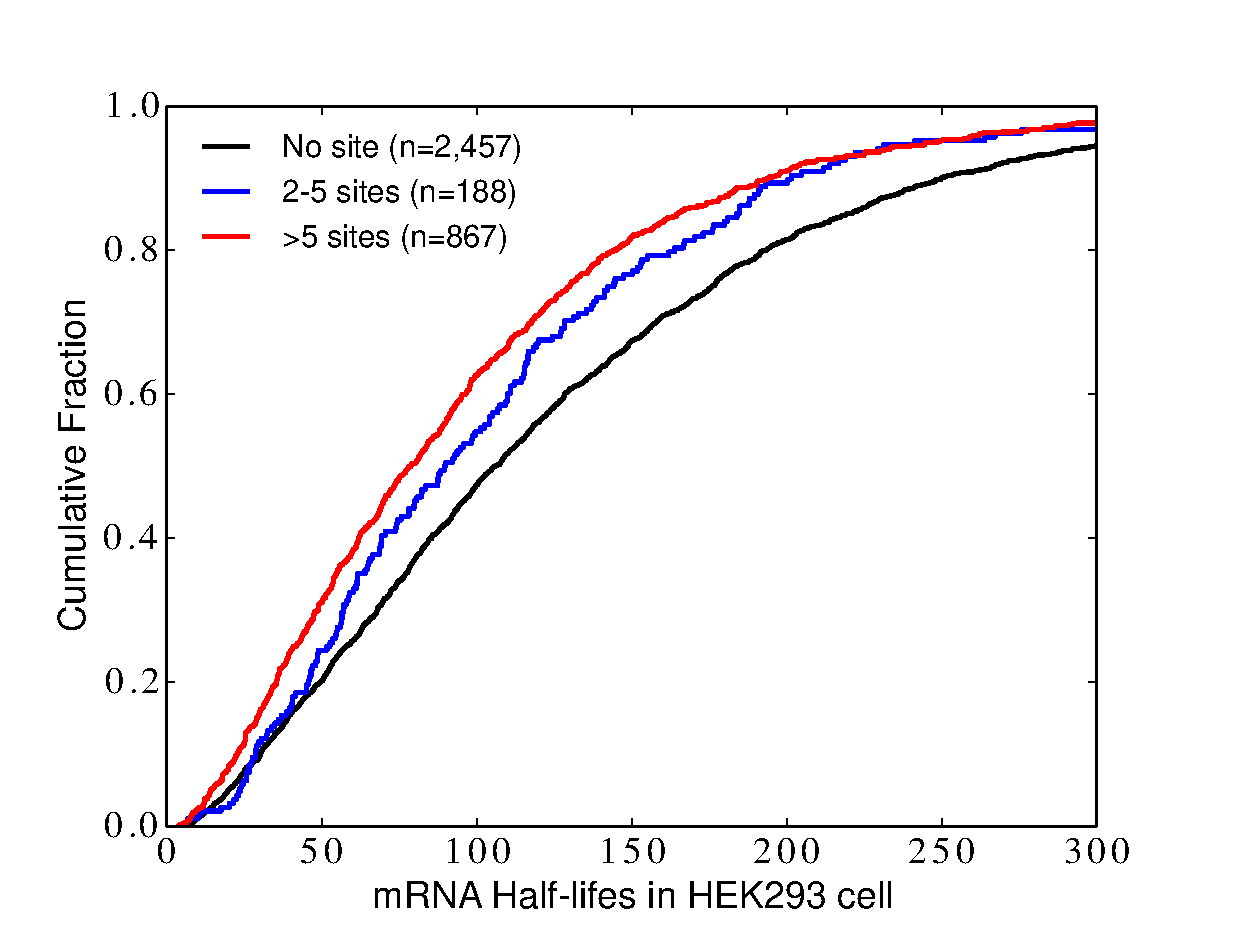
\includegraphics[width=0.7\textwidth,clip]{ch4_results_discussion/figures/pum_plus_intmiRNAs_number_of_sites}

\caption[Effect of binding sites of PUM1(2) and its interacting miRNAs count on expression of transcripts]{Functional effect of number of PUM1(2) and its interacting miRNA sites on transcripts. Transcripts with more binding sites of PUM1(2) and its interacting miRNAs have significantly shorter half-lives compared to other transcripts.}
\label{PUM_number_of_sites}
\end{figure}
%\shorthandon{=}

Figure \ref{PUM_number_of_sites} shows the differences between these groups. We observe that transcripts in group three have shorter half-lives compared to those transcripts with two up to five sites and also those with no PUM1(2) sites at all (P-values = $0.03$ and $7.91E-20$ respectively). This analysis demonstrates that the more PUM1(2) and its interacting miRNAs sites exist in a transcript, the higher possibility there is that it will downregulate faster.

\subsection{The effect of distance between binding sites of PUM1(2) on stability of mRNAs}

It is also clear from the figure \ref{PUM_qvalue_heatmap} that PUM1 binding sites are close to each other. Q-values are significant in 150nt up and down stream of the PUM1 binding sites when we consider its own sites as interacting factors. We suppose that this is because PUM1(2) interacts with itself. In order to further investigate this issue, we analyzed the effect of number of PUM1(2) binding sites on transcripts stability. Also we assessed the difference between two conditions in which PUM1(2) binding sites co-occur in close ranges whereas they are not close to each other.

In order to investigate our hypothesis, first we need to classify sites as \textit{close} and \textit{not close} to each other. We determined two sites as \textit{close} to each other when there was at most 50 nucleotides between the starting position of those sites, otherwise we considered them as \textit{not close}. The reason for considering this threshold is that we are trying to focus on those PUM1(2) sites which are inside same stem loop otherwise they will be unlikely to cooperate with each other. We classified transcripts into three groups: (i) those that do not contain any PUM1(2) sites. (ii) those that contain two or more PUM1(2) sites and there is at least two sites which are close to each other. (iii) those that contain two or more PUM1(2) sites but none of them are close to each other. Figure \ref{pum_close_not_close} shows the mRNA half-life measurement in HEK293 cells for these three groups. We observe that transcripts with more than two sites (close) have significantly shorter half-lives compared to those with more than two sites but with no close sites (not close) (P-value = $2.98E-05$). Besides, both first and second groups have significantly shorter half-lives compared to the transcripts with no PUM1(2) sites at all (P-values = $1.04E-22$ and $2.6E-04$ respectively). This observation represents that transcripts with close PUM1(2) sites tend to have shorter half-lives and the reason for this is likely because PUM1(2) binding sites are cooperatively interacting with each other.

%\shorthandoff{=}
\begin{figure}[H]
	\centering
	\subfloat[]{
	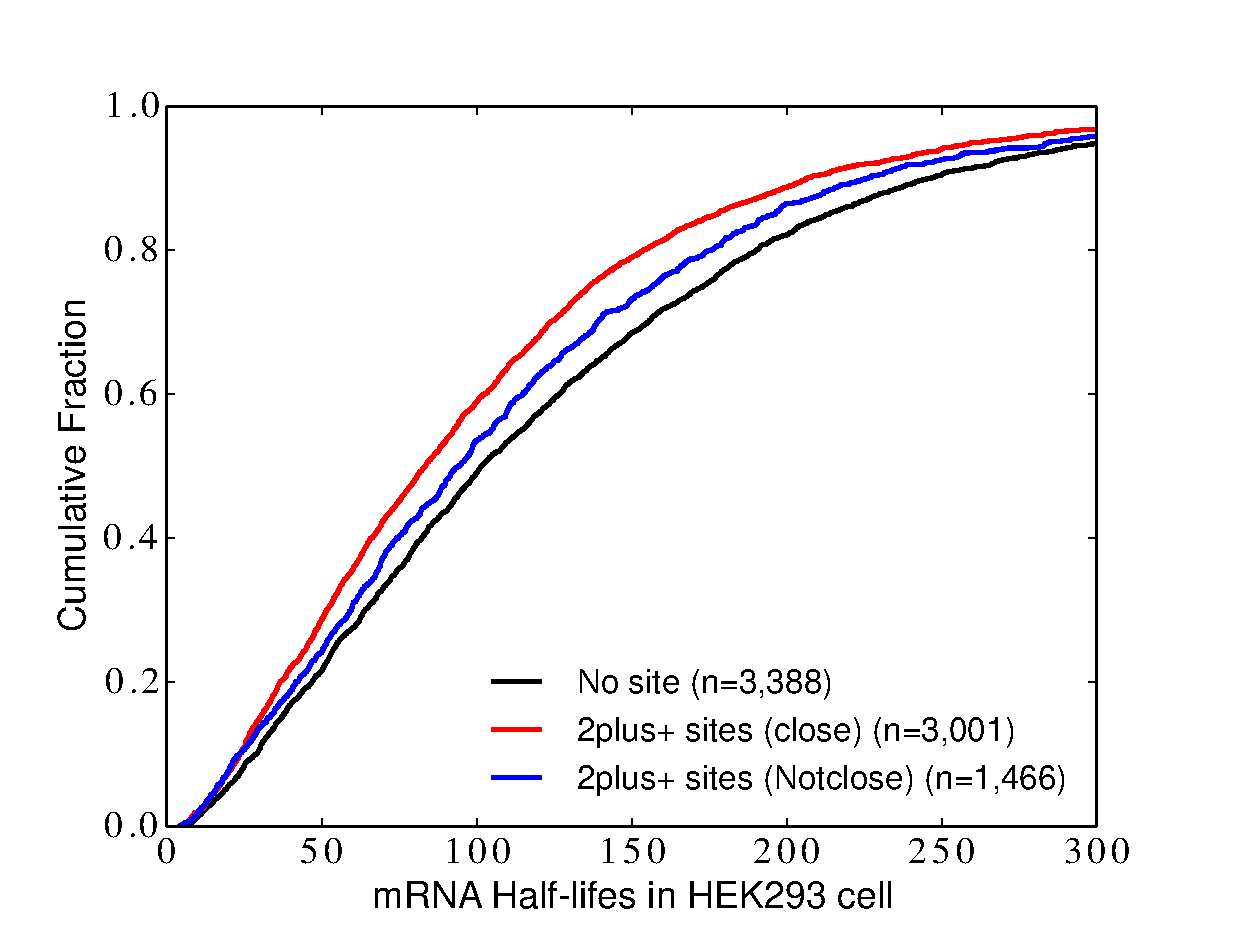
\includegraphics[width=0.9\textwidth,clip]{ch4_results_discussion/figures/pum_close_notclose}
    \label{pum_close_not_close}
}
\caption[Effect of close and not close PUM binding sites on expression of transcripts]{Functional effect of close PUM1(2) sites on stability of mRNAs. Transcripts where PUM1(2) binding sites are close to each other have significantly shorter half-lives compared to other transcripts where there are no close PUM1(2) sites.}
\end{figure}
%\shorthandon{=}

Although the result for this analysis shows that transcripts with close PUM1(2) sites are destabilizing faster than those with no close PUM1(2) sites at all. However, the disadvantage of this analysis is that we ignore the fact that this difference may be not clearly because of interaction between close PUM1(2) sites. Actually when we compare the transcripts in first and second groups, we are not clearly sure that the difference is due to the phenomenon of close sites. It might be related to the number of PUM1(2) sites. One solution is to restrict the number of PUM sites and then re-plot the figure but it leads to data loss and weakens the output. Another solution is to distinguish the results according to number of close sites. However, this time we should make number of sites restrict. Actually, there are two variables here, number of sites and number of close sites. In order to get a better result, we should take these two variables in to consideration at the same time. However, this approach reduces the transcripts count and makes the result not reliable. In the future, we may reintroduce this analysis for larger group of transcripts to get much more reliable result.

\clearpage
\section{Predicting stability and gene expression with a logistic regression model}

In this analysis, we took into account the effect of multiple factors to predict stability and gene expression levels. Figure \ref{zhao_nostr_nogparclip} compares the AU-ROC curves of three models that predict half-life or steady-state mRNA abundance in Zhao dataset: (i) \textit{miRNAs}, \textit{activators} and \textit{repressors} are used as features (miRNAs + RBPs); (ii) counts of 16 2-mers that represent dinucleotide content are used as features (dinucleotide content); (iii) the combination of features used in model (i) and (ii) are used (dinucleotide content + miRNAs + RBPs). 

%\shorthandoff{=}
\begin{figure}[H]
	\centering
	\subfloat[]{
	\includegraphics[width=0.6\textwidth,clip]{ch4_results_discussion/figures/Figure7a}
    \label{zhao_halflife_nostr_nogparclip}
}
\quad
	\subfloat[]{
    \includegraphics[width=0.6\textwidth,clip]{ch4_results_discussion/figures/Figure7b}
    \label{zhao_steady_nostr_nogparclip}
}

\caption[Predicting stability and gene expression with a logistic regression model]{Results of predicting half-life and steady-state mRNA levels in Zhao dataset.  \subref{zhao_halflife_nostr_nogparclip} ROC curves (interpolation of 100 curves) of models that predict half-life in Zhao dataset, area shows the average of 100 AU-ROC values. \subref{zhao_steady_nostr_nogparclip} ROC curves (interpolation of 100 curves) of models that predict steady state mRNA abundance in Zhao dataset, area shows the average of 100 AU-ROC values. }
\label{zhao_nostr_nogparclip}
\end{figure}
%\shorthandon{=}

We observe that dinucleotide features alone perform much better than features formed from sites of miRNAs and RBPs (Wilcoxon signed-rank test applied to 100 AU-ROCs from two models, P-value = $6.0E-18$ for half-life and P-value = $2.5E-17$ for mRNA abundance); however, the addition of miRNA and RBP features on top of dinucleotide content features improves the predictive power of the model (P-value = $1.1E-17$ for half-life and P-value = $9.1E-18$ for mRNA abundance). %Fitted parameter values can be seen in Supplementary Figure 1.

%\shorthandoff{=}
\begin{figure}[H]
	\centering
	\subfloat[]{
	\includegraphics[width=0.65\textwidth,clip]{ch4_results_discussion/figures/Figure8a}
    \label{schueler_halflife_HEK293_500}
}
\quad
	\subfloat[]{
    \includegraphics[width=0.65\textwidth,clip]{ch4_results_discussion/figures/Figure8b}
    \label{schueler_halflife_MCF7_500}
}
\caption[Optional caption for list of figures]{Results of predicting half-life in HEK293 and MCF7 cells (Schueler dataset)  \subref{schueler_halflife_HEK293_500}  ROC curves (interpolation of 100 curves) of models that predict half-life in HEK293 cells, area shows the average of 100 AU-ROC values.  \subref{schueler_halflife_MCF7_500} ROC curves (interpolation of 100 curves) of models that predict half-life in MCF7 cells, area shows the average of 100 AU-ROC values.}
\label{Schueler_halflife_nostr_nogparclip}
\end{figure}
%\shorthandon{=}

We repeated the same analysis with half-life datasets in HEK293 and MCF7 cells (Schueler dataset) this time calculating features considering the 3'UTRs of the transcripts. Figure  \ref{schueler_halflife_HEK293_500} and \ref{schueler_halflife_MCF7_500} show the ROC curves of the logistic regression models predicting half-life in HEK293 and MCF7 cells, respectively. For both cell types, the increase in AU-ROC between model(i) and model(ii); and between model(ii) and model(iii) is significant according to Wilcoxon signed-rank test (P-values are $1.9E-12$ and $9.0E-12$ for HEK293 cells and $6.8E-05$ and $2.7E-13$ for MCF7 cells). 

We also checked whether our features simply represent a bias of 3'UTR length. The 3'UTR segments in Zhao dataset are all of the same length whereas the Schueler dataset contains 3'UTRs of variable length. Predicting half-life with only 3'UTR length in HEK293 and MCF7 cells results in a mean AU-ROC value of 0.545 and 0.548, respectively. This confirms that our features do not simply represent 3'UTR length.

In addition to counting simply the number of binding sites as above, we also tried using more advanced features. For instance, we used the sum of the accessibility of sites of \textit{miRNAs}, \textit{activators} or \textit{repressors} as features. We also tried considering only gPARCLIP- or CLIP-supported RBP sites and miRTarBase or Ago2-CLIP supported miRNA sites. Lastly, we took into account the effect of competition by counting the sites that overlap with other factors' sites as 0.5 rather than 1. However, neither of these modifications resulted in improved performance in Zhao or Schueler datasets (data not shown).